\documentclass[APA,STIX1COL]{WileyNJD-v2}
\usepackage{siunitx}
\usepackage{graphicx}
\usepackage{subcaption}
\usepackage{float}        % for [H] placement

\articletype{Research Article} % Specify article type

\received{Date Month Year}
\revised{Date Month Year}
\accepted{Date Month Year}
\copyyear{2025}
\startpage{1}

\raggedbottom

%%%%%%%%%%%%%%%%%%%%%%%%%%%%%%
% My commands:
\newcommand{\bruno}[1]{\textcolor{blue}{#1}} % Bruno Sanso edits - blue
\newcommand*\mymin[1][]{\min_{#1}\,}
\newcommand{\vect}[1]{\mathbf{#1}}  
\newcommand\numberthis{\addtocounter{equation}{1}\tag{\theequation}}
\newcommand\independent{\protect\mathpalette{\protect\independenT}{\perp}}
\def\independenT#1#2{\mathrel{\rlap{$#1#2$}\mkern2mu{#1#2}}}
%%%%%%%%%%%%%%%%%%%%%%%%%%%%%%

\begin{document}

\title{Bayesian Quantile-Based Correction and Synthesis of River Flow Forecasts\protect\thanks{This research was conducted as part of the PhD dissertation of the first author at the University of California, Santa Cruz.}}

\author[1]{Antonio Aguirre*}
\author[1]{Raquel Prado}
\author[1]{Bruno Sans\'o}

\authormark{Aguirre \textsc{et al.}} % Running head author name

\address[1]{\orgdiv{Department of Statistics}, \orgname{University of California, Santa Cruz}, \orgaddress{\state{California}, \country{USA}}}

\corres{*Corresponding author: Antonio Aguirre. \email{jaguir@ucsc.edu}}

\presentaddress{University of California, Santa Cruz, Santa Cruz, CA, USA.}

\abstract[Summary]{Accurate uncertainty quantification and forecasting of dynamic environmental phenomena, such as river flow, are critical for effective resource management and disaster mitigation. Existing forecasting methods often fail to adequately characterize uncertainty during extreme events, including floods and prolonged droughts, leading to significant challenges in preparedness and response. We address these limitations by developing fast, adaptive methods that utilize Dynamic Quantile Linear Models (DQLMs). We propose a coherent modeling framework that integrates historical river flow data with environmental and climatological information, along with historical analysis and prediction outputs from various climate agencies. Our work corrects forecast uncertainty at various quantile levels and combines posterior predictive information from various models. The methodology is motivated by the analyses and medium-range forecasting of river flow for the San Lorenzo River, a vital water resource for the Santa Cruz region in California, USA.}

\keywords{Bayesian forecasting, quantile regression, dynamic models, river flow prediction}

\jnlcitation{\cname{%
\author{Aguirre A.}, 
\author{Prado R.}, and 
\author{Sans\'o B.}} (\cyear{2025}), 
\ctitle{Bayesian quantile-based correction and synthesis of river flow forecasts}, \cjournal{Environmetrics}, \cvol{XX:1--20}.}

\maketitle

\footnotetext{\textbf{Abbreviations:} CRPS, Continuous Ranked Probability Score; DQLM, Dynamic Quantile Linear Model.}


\section{INTRODUCTION}

Accurate forecasting of river flow dynamics is crucial for regions such as Santa Cruz, CA, which rely on precipitation with a pronounced seasonal pattern to sustain essential resources, including water supply, ecological balance, and flood management. The ability to predict extreme events, such as floods and droughts, is vital for minimizing economic losses and enhancing water resource planning. However, forecasting river flow poses significant challenges due to the complexity of the physical processes governing hydrological systems, which continuously interact with a variety of environmental factors. Prediction uncertainty arises from several sources, including incomplete model's initial conditions, missing data, observational inaccuracies, and errors introduced during data assimilation. Furthermore, limitations in the spatial and temporal resolution of models, parameter simplifications, and variability in boundary conditions exacerbate these uncertainties. The inherently chaotic nature of hydrological systems, characterized by unstable flow patterns and complex dynamics, further compounds these challenges. Foundational insights into ensemble prediction uncertainties are provided by \citet{buizza2005comparison}, while recent studies by \citet{tarek2021daily} and \citet{thiboult2016accounting} explore uncertainty quantification and mitigation strategies in hydrological forecasting.

Hydrological predictions are often produced using physical models that simulate the behavior of hydrological and meteorological systems. These models rely on numerical approximations to represent key physical processes such as precipitation, evaporation, and runoff. Quantifying prediction uncertainty has become a significant focus of research, as it is critical for evaluating forecast reliability and informing effective decision-making \citep{kim2019hybrid, haiden2021evaluation, hughes2024evaluation, wu2020ensemble}. A prominent probabilistic approach, ensemble forecasting, generates multiple forecast scenarios by perturbing initial conditions or varying model parameters. Although ensemble forecasting has shown promise, challenges remain, particularly the underdispersion of ensemble members, which leads to an incomplete representation of uncertainty. Techniques such as the Singular Vector (SV) method \citep{buizza1999stochastic} and Stochastically Perturbed Parameterization Tendencies (SPPT) \citep{SPPT, leutbecher2017stochastic} have been developed to address these limitations and have been successfully integrated into operational systems.

Despite these advances, accurate quantification of uncertainty for forecasts of complex geophysical systems remains an open problem and an active area of research. In operational hydrological forecasting, agencies collaborate with research institutions to provide real-time streamflow ensemble forecasts. These forecast products vary widely in terms of their forecast horizons (short, medium, or long-range), spatial resolutions, input data (e.g., meteorological estimates), and the data assimilation techniques employed. Integrating these diverse forecast products into cohesive frameworks presents a significant challenge. We consider two forecast products that exemplify these complexities: the European Centre for Medium-Range Weather Forecasts (ECMWF) ensemble \citep{molteni1996ecmwf, isaksen2010ensemble, haiden2021evaluation} and advancements from the National Weather Service (NWS) and the National Oceanic and Atmospheric Administration (NOAA) \citep{kim2019hybrid, demargne2013science, barlage2021importance, johnson2023comprehensive}.

The integration of different forecast products requires advanced methodologies capable of effectively synthesizing information across spatial, temporal, and probabilistic dimensions. One promising avenue lies in forecast blending, a form of statistical post-processing, which utilizes statistical models to combine multiple forecast sources to improve overall predictive accuracy and uncertainty quantification. Comprehensive recent reviews on forecast combination are available in \citet{siegert2019forecast, vannitsem, wang2022forecastcombinations50yearreview}. Among these, Bayesian approaches have gained significant attention due to their ability to coherently account for uncertainty while incorporating prior knowledge and dynamically updating forecasts as new information becomes available. For Bayesian forecast blending methodology, refer to \citet{duan2006bma, yumnam2022quantile, aastveit2022quantifying, du2018ensemble_forecasting, doubleday, kleiber2011geostatistical, mcalinn2019dynamic, tallman2023bayesianpredictivedecisionsynthesis, johnson2023bayesian}. Spatial forecast blending applications are discussed in \citet{salazar2011comparing, beltran, berre2007variational, kleiber2011geostatistical}. For spatio-temporal forecast blending, see \citet{hemri2020multi, ascmo-6-79-2020}. 

Our work focuses on advancing uncertainty quantification and improving forecast accuracy in hydrology, with potential extensions to other fields where both retrospective and forecasting products are widely available. Hydrological forecasts, particularly during extreme events such as floods and prolonged droughts, often face challenges in representing uncertainty, limiting their reliability and applicability. Using recent approaches in the area of Dynamic Quantile Linear Models (DQLMs) \citep{goncalves, gourieroux2008dqlm, barata2021_flex_quantile}, we address these limitations by developing methods specifically designed to quantify uncertainty in such scenarios.

A key contribution of this work lies in the development of scalable Bayesian methods that extend posterior inference techniques for DQLMs. By addressing challenges associated with non-conjugate parameters, we utilize Laplace-Delta techniques as proposed in \citet{wang2013nonconjugatevb}, enabling robust and efficient inference. These advances overcome the computational limitations inherent in the Importance-Sampling techniques used in \citet{barata2021_flex_quantile}, resulting in fast and scalable Variational Bayes (VB) algorithms. The proposed methods facilitate the dynamic quantile analysis of large temporal datasets, allowing the identification of long-term trends and critical behaviors with significant scientific and practical implications.

In addition to improving inference techniques, we propose a framework for integrating diverse climate-agency-generated products that combines retrospective analyses and forecast ensembles within a coherent Bayesian framework. Motivated by insights into the practices of forecasting agencies, which often rely on retrospective analyses to refine forecast accuracy \citep{vannitsem, haiden2021evaluation, abdelkader2023assessing}, our methodology leverages discrepancies between retrospective products and observations to correct forecast products systematically. This approach not only improves hydrological forecasting, but is adaptable to other domains where historical data and climate agency products are abundant and available but challenging to integrate. 

Finally, we combine posterior predictive outputs from multiple models used to estimate different quantiles. This ensures the integration of all posterior predictive distributions, merging model outputs with different objectives to provide unified uncertainty quantification for both historical and forecasting periods. 

The remainder of the paper is organized as follows. Section~\ref{sec:methodology} outlines the methodology, including the development and application of Dynamic Quantile Linear Models, the integration of retrospective and forecast products, prior specifications, and posterior inference algorithms. Section~\ref{sec:data} describes the San Lorenzo River flow observations and the climate agency forecast products used in this study. In Section~\ref{sec:results}, we present the results of the analysis, including predictions for multiple quantiles,  correction of forecast biases, and synthesis of forecasting products. Finally, Section~\ref{sec5} provides concluding discussion.

\section{METHODOLOGY}
\label{sec:methodology}

We first introduce some notation to be used throughout the article. We use bold uppercase letters (e.g., $\mathbf{W}, \mathbf{F}, \mathbf{G}$) to denote matrices, and bold lowercase letters (e.g., $\mathbf{x}, \mathbf{\psi}, \mathbf{\theta}$) to denote vectors. We denote the identity matrix of dimension $m \times m$ as $\mathbf{I}_m$, a vector of zeros of dimension $m \times 1$ as $\mathbf{0}_m$, and a vector of ones of dimension $m \times 1$ as $\mathbf{1}_m$.

\subsection{Flexile Quantile Estimation: The Extended Asymmetric Laplace}
\label{subsec:exal}

The use of the Asymmetric Laplace (AL) distribution for quantile inference within a Bayesian framework is well-established with both empirical and theoretical justifications \citep{yu2001bayesian, sriram2013theoretical}. We use a recent extension of the AL distribution, which we refer to as the extended asymmetric Laplace (exAL), that addresses intrinsic issues for the AL working likelihood, such as the limitations imposed by its skewness. \citet{yan2025new} proposed the extended asymmetric Laplace (exAL) distribution, $\text{exAL}_{p_0}(\mu, \sigma, \gamma)$, where $\mu$ represents the $p_0$th quantile of interest, $\sigma$ is a positive scale parameter, and $\gamma$ is the skewness parameter. Moreover, the parameter $\gamma$ has bounded support over the interval $(L, U)$, where $L$ is the negative root of $g(\gamma) = 1 - p_0$ and $U$ is the positive root of $g(\gamma) = p_0$, with $g(\gamma) = 2 \Phi(-|\gamma|) \exp(\gamma^2 / 2)$ and $\Phi$ denoting the standard normal CDF. To improve the efficiency of our posterior sampling algorithms, we utilize the extended stochastic representation of an exAL random variable described in \citet{yan2025new}. That is, if $y \sim \text{exAL}(\mu, \sigma, \gamma)$, then there exist independent random variables $\epsilon \sim \mathcal{N}(0, 1)$, $z \sim \text{Exp}(1)$, and $s \sim \mathcal{N}^+(0, 1)$, (where $\mathcal{N}^+(0, 1)$ denotes the standard normal distribution truncated to the positive real line), such that  \( y = \mu + C(\gamma; p_0)\sigma |\gamma| s + A(\gamma; p_0) \sigma z + \sqrt{B(\gamma; p_0) \sigma^2 z} \cdot \epsilon, \) where $A(\gamma; p_0) = \frac{1 - 2 p(\gamma; p_0)}{p(\gamma; p_0) \, [1 - p(\gamma; p_0)]}$, $B(\gamma; p_0) = \frac{2}{p(\gamma; p_0) \, [1 - p(\gamma; p_0)]}$, $C(\gamma; p_0) = [I(\gamma > 0) - p(\gamma; p_0)]^{-1}$, and $p(\gamma; p_0) = I(\gamma < 0) + \{p_0 - I(\gamma < 0)\} / g(\gamma)$.


\subsection{The Extended Dynamic Quantile Linear Models} 
\label{sec:dqlm}

Our core model is an extended Dynamic Quantile Linear Model (exDQLM), introduced by \citep{barata2021_flex_quantile}, which results from the temporal extension of the exAL. We define \textbf{Model A}, for \( 1 \leq t \leq T \) as:
\begin{align}
      \text{Output}:&& y^o_t | \boldsymbol{\theta}_t, \zeta_t, \sigma^o, \gamma^o &\sim \text{exAL}_{p_0} \Big( \mathbf{F}'_t \boldsymbol{\theta}_t + \zeta_t, \sigma^o, \gamma^o \Big) \label{A1} \\
    \text{Trend and Seasonal States}:&& \boldsymbol{\theta}_t | \boldsymbol{\theta}_{t-1} &\sim \mathcal{N} \Big( \mathbf{G}_t \boldsymbol{\theta}_{t-1}, \mathbf{W}^\theta_t \Big) \label{A2} \\
    \text{Cumulative Effect State}:&& \zeta_t | \zeta_{t-1}, \bm{\psi}_t &\sim \mathcal{N} \Big( \lambda \zeta_{t-1} + \mathbf{x}'_t \boldsymbol{\psi}_t, \text{w}^\zeta_t \Big) \label{A3} \\
    \text{Exogenous Effects States}:&& \boldsymbol{\psi}_t | \boldsymbol{\psi}_{t-1} &\sim \mathcal{N} \Big( \boldsymbol{\psi}_{t-1}, \mathbf{W}^\psi_t \Big). \label{A4}
\end{align} 

\noindent Here, $T$ denotes the length of the series considered, $y^o_t \in {\mathbb{R}}$ denotes the observed river flow at time $t$, $\mathbf{F}_t \in {\mathbb{R}^{\text{p}}}$ denotes the observational vector, $\boldsymbol{\theta}_t \in {\mathbb{R}^{\text{p}}}$ denotes the state vector, $\sigma^o>0$ denotes the scale parameter, and $\gamma^o \in [L, U]$ denotes the skewness parameter, where $L$ and $U$ depend on $p_0$ as defined above. The state vector follows a linear evolution, described by the evolution matrix $\mathbf{G}_t \in {\mathbb{R}^{\text{pxp}}}$ and error with covariance matrix $\mathbf{W}^{\theta}_t \in {\mathbb{R}^{\text{pxp}}} $. 
We use a transfer function to incorporate relevant information from external sources, denoted, at time $t$, as $\mathbf{x}_t \in {\mathbb{R}^{\text{m}}}$. The term \( \zeta_t \in {\mathbb{R}} \) denotes the total accumulated effect at time \( t \) of such covariates, whose effects are denoted by \( \boldsymbol{\psi}_{t} \in {\mathbb{R}^{\text{m}}} \),  an $m$-dimensional vector, whose $i$-th component we will denote as $\psi_{i,t}$, and with covariance $\mathbf{W}^{\psi}_t \in {\mathbb{R}^{\text{mxm}}} $. Notice that $\zeta_t$ centers around the sum of the total immediate effect, $\mathbf{x}'_t \boldsymbol{\psi}_t$ and at a fixed proportion, $\lambda$,  of the previous total accumulated effect. Refer to \citet{barata2021_flex_quantile} for further discussion of transfer functions.

Rewriting the transfer function component, a compact representation of \textbf{Model A} using the previous notation can be expressed as follows. For  \( 1 \leq t \leq T \):
\begin{align}
    \text{Output}:&& y^o_t | \boldsymbol{\alpha}_t, \sigma^o, \gamma^o & \sim exAL_{p_0} \Big( \Tilde{\mathbf{F}}'_t \boldsymbol{\alpha}_t, \sigma^o, \gamma^o \Big) \label{A5} \\
    \text{All States}:&& \boldsymbol{\alpha}_t | \boldsymbol{\alpha}_{t-1} &\sim \mathcal{N} \Big( \Tilde{\mathbf{G}}_t \boldsymbol{\alpha}_{t-1}, \Tilde{\mathbf{W}}_t \Big), \label{A6} 
\end{align} 
where,  \( \, \boldsymbol{\alpha}_t = \begin{bmatrix} 
        \boldsymbol{\theta}_t \\ \zeta_t \\ \boldsymbol{\psi}_t 
    \end{bmatrix},  \) \,  
    \( \Tilde{\mathbf{F}}_t = \begin{bmatrix} 
        \mathbf{F}_t \\ \mathbf{F}^{\text{trans}}_t 
    \end{bmatrix}, \) \, 
    \( \mathbf{F}^{\text{trans}}_t = \begin{bmatrix}
        1 \\ \mathbf{0}_{m}
    \end{bmatrix},  \) \,  
    \( \Tilde{\mathbf{G}}_t = \text{BlockDiag} \Big( \mathbf{G}_t, \mathbf{G}^{\text{trans}}_t \Big), \, \) 
    \( \mathbf{G}^{\text{trans}}_t = \begin{bmatrix}
        \lambda & \mathbf{x}'_t \\
        \mathbf{0}_{m} & \mathbf{I}_m
    \end{bmatrix}, \) \, 
    \newline 
    and \( \, \Tilde{\mathbf{W}}_t = \text{BlockDiag} \Big( \mathbf{W}^\theta_t, \text{w}^\zeta_t, \mathbf{W}^\psi_t \Big). \)
    
\subsection{Incorporating retrospective products}
\label{subsec:retrospective}

Retrospective analyses, often referred to as reanalyses, are gridded climate and hydrological products generated by climate agencies through the consistent application of a deterministic model over an extended historical period. Unlike real-time forecasts, these products assimilate all available past observations into the model, benefiting from complete datasets, improved calibration, and stable boundary conditions. The resulting fields represent a physically consistent reconstruction of past atmospheric or hydrological states, typically at high spatial and temporal resolution. Retrospective products are widely used for model validation, bias correction, and the calibration of forecasting systems, as they provide a benchmark dataset that is free from the flow-dependent uncertainties and observational gaps that affect real-time forecasts. In hydrology, they are particularly valuable for understanding long-term variability, assessing extreme events, and informing post-processing techniques that aim to improve the accuracy of operational forecast products.

We extend \textbf{Model A} as expressed in \eqref{A5} and \eqref{A6} in to incorporate $J\geq1$ retrospective analyses as follows.  We define \textbf{Model B}, for \( 1 \leq t \leq T \) as:
\begin{align}
      \text{Output}:&& y^o_t | \boldsymbol{\alpha}_t, \sigma^o, \gamma^o &\sim exAL_{p_0} \Big( \Tilde{\mathbf{F}}'_t \boldsymbol{\alpha}_t, \sigma^o, \gamma^o \Big) \label{B1}  \\
    \text{Retrospective}:&& z^j_t | \boldsymbol{\alpha}_t, \boldsymbol{\delta}^j_t, \sigma^j, \gamma^j &\sim exAL_{p_0} \Big( \Tilde{\mathbf{F}}'_t \boldsymbol{\alpha}_t + \mathbf{F}'_t \boldsymbol{\delta}^j_t, \sigma^j, \gamma^j \Big), \quad 1 \leq j \leq J \label{B2} \\
    \text{All states in } \textbf{Model A}:&&\boldsymbol{\alpha}_t | \boldsymbol{\alpha}_{t-1} &\sim \mathcal{N} \Big( \Tilde{\mathbf{G}}_t \boldsymbol{\alpha}_{t-1}, \Tilde{\mathbf{W}}_t \Big) \label{B3}\\
    \text{Discrepancy States}:&& \boldsymbol{\delta}^j_t | \boldsymbol{\delta}^j_{t-1} &\sim \mathcal{N} \Big( \boldsymbol{\mathbf{G}}_t \boldsymbol{\delta}^j_{t-1}, \mathbf{W}^{\delta^j}_t \Big), \quad 1 \leq j \leq J. \label{B4}
\end{align} 
Here, \( z^{j}_t \in {\mathbb{R}} \), denotes the retrospective analysis from the \( j \)-th forecasting agency at time \( t \), and $\boldsymbol{\delta}^j_t \in {\mathbb{R}}^J$ denotes the forecasters' quantile-discrepancy state vector, whose \( r \)-th component is denoted by $\delta^{j,r}_t$. As in \textbf{Model A}, the term \( \Tilde{\mathbf{F}}'_t \boldsymbol{\alpha}_t \) represents the $p_0$-th quantile at time \( t \) for the USGS measurements, and can be also expressed as \( \mathbf{F}'_t \boldsymbol{\theta}_t + \zeta_t \) as in \eqref{A1}.  Moreover, in \eqref{B2}, $\Tilde{\mathbf{F}}'_t \boldsymbol{\alpha}_t+\mathbf{F}'_t \boldsymbol{\delta}^j_t $ represents the quantile at the $p_0$-th level for the \( j \)-th retrospective analysis, and can be rewritten as $ \mathbf{F}'_t ( \boldsymbol{\theta}_t+\boldsymbol{\delta}^j_t ) + \zeta_t$.  This last expression highlights the role of $\boldsymbol{\delta}^j_t$ as the parameter vector that corrects for component-specific discrepancies with respect to the state $\boldsymbol{\theta}_t$. The motivation of endowing the discrepancy term with a structured dynamic as described in \eqref{B4} is twofold. First, it allows for a richer analysis of the observed discrepancies between climate agency estimates and measurements than when modeled as a constant. For example, a climate agency's retrospective analysis might show smaller discrepancies with respect to the measurements during dry seasons, while their discrepancies might be larger during rainy seasons. Second, the further correction of forecast ensembles, discussed in Subsection~\ref{subsec:ensemble}, depends on our ability to learn the  behavior of the discrepancies over time and spread them into the future. For similar blending techniques using discrepancies in forecast products, see \cite{salazar2011comparing,beltran} 
and \cite{lemos2009spatio}. In addition, we consider \( \sigma^j > 0\) and \( \gamma^j \in [L, U]\), for $j \in \{0, 1, ..., J \}$ denoting the scale and skewness parameters, respectively. Each pair (\( \sigma^{(\cdot)}, \gamma^{(\cdot)} \)) is specific to a particular data source, either the observed measurements or the retrospective analysis from a given agency. We model these parameters separately because retrospective products from different climate agencies are generated using distinct methodologies, leading to differences in scale and shape that are difficult to capture with a single shared pair of parameters. This approach aims to aid the model to account for source-specific variability and improve the accuracy of quantile estimation and uncertainty quantification across all sources.

Furthermore, a more compact representation of \textbf{Model B} for \(1 \leq t \leq T\) can be expressed using previous notation as follows:
\begin{align}
     \text{Output}:&& y^o_t | \boldsymbol{\mu}_t, \sigma^o, \gamma^o &\sim exAL_{p_0} \Big( \textbf{h}_{t,1}' \boldsymbol{\mu}_t, \sigma^o, \gamma^o \Big) \\ \label{B5}
    \text{Retrospective}:&& z^j_t | \boldsymbol{\mu}_t, \sigma^j, \gamma^j &\sim exAL_{p_0} \Big( \textbf{h}_{t,j+1}' \boldsymbol{\mu}_t, \sigma^j, \gamma^j \Big), \quad 1 \leq j \leq J \\ \label{B6}
    \text{All states}:&& \boldsymbol{\mu}_t | \boldsymbol{\mu}_{t-1} &\sim \mathcal{N} \Big( \boldsymbol{D}_t \boldsymbol{\mu}_{t-1}, \boldsymbol{\Lambda}_t \Big),  \label{B7}
\end{align} 
where, \(  \boldsymbol{\mu}_t = \begin{bmatrix} \boldsymbol{\theta}_t \\ \boldsymbol{\delta}_t \\ \zeta_t \\ \boldsymbol{\psi}_t \end{bmatrix}, \,
\textbf{H}_t &= \begin{bmatrix} 
    \mathbf{F}_t & \begin{bmatrix} \mathbf{F}_t \stackrel{J \; \text{times}}{\dots} \mathbf{F}_t \end{bmatrix} \\
    \mathbf{0}_{pJ} &  \text{BlockDiag} \big( \mathbf{F}_t, \stackrel{J \; \text{times}}{\dots}, \mathbf{F}_t  \big) \\
    1 & \mathbf{1}_{J}' \\
    0 & \mathbf{0}_{J}'
\end{bmatrix}, \,
\boldsymbol{D}_t = \text{BlockDiag} \Big( \mathbf{G}_t, \stackrel{J+1 \; \text{times}}{\dots}, \mathbf{G}_t, \mathbf{G}^{\text{trans}}_t \Big), \newline
\boldsymbol{\Lambda}_t = \text{BlockDiag} \Big( \mathbf{W}^\theta_t, \mathbf{W}^{\delta^1}, \dots, \mathbf{W}^{\delta^J}_t, w^\zeta_t, \mathbf{W}^{\boldsymbol{\psi}}_t \Big) 
\). Here, $\textbf{h}_{t,k}$ denotes the k-th column of $\boldsymbol{\text{H}}_t$, and  \( \boldsymbol{\delta}_t \in {\mathbb{R}}^{pJ} \) denotes all $J$  concatenated discrepancy vectors at time $t$. It is important to highlight the conditional independence assumption between \( y^o_t \), the observed measurement, and the retrospective analysis \( z^{j}_t \), as well as between retrospective analyses. This assumption simplifies the modeling process but can be relaxed to account for correlations between these variables, providing a more comprehensive understanding of the relationships between observations and climate agency analyses. Such correlated extension can be addressed by the exDQLM multivariate extension proposed by \citet{barata2021dqlm}.

\subsection{Incorporating Ensemble Forecasts}
\label{subsec:ensemble}

Ensemble forecast products are real-time predictive datasets generated by climate and hydrological agencies using numerical models initialized with the most recent observations. Rather than producing a single deterministic forecast, ensemble systems run the model multiple times with perturbed initial conditions and/or model parameters, generating a set of trajectories that collectively represent forecast uncertainty. Each ensemble member reflects a plausible future evolution of the system, allowing forecasters to estimate probabilities of events, quantify uncertainty, and assess forecast reliability. In hydrology, ensemble forecasts are widely used for flood risk assessment, reservoir management, and water resource planning, providing decision-makers with probabilistic information that complements deterministic outlooks.

We extend \textbf{Model B} to a forecasting period, $t>T$, by incorporating the forecast ensemble products as follows. We denote \(K_{(j)}\) as the horizon length of the forecasts produced by the $j$-th forecaster, and assume we order the forecasters by horizon length, that is \(K_{(1)} \geq \ldots \geq K_{(J)} \). Moreover, assume the $j$-th forecaster's ensemble comprises $I_j \geq 1$ members. And denote the $j$-th forecaster $i$-th ensemble member $k$-step-ahead prediction generated at time $T$ as $y^{j,i}_T(k) \in {\mathbb{R}}$. We define \textbf{Model C} as \textbf{Model B} for $t \leq T$, and for the forecasting period, $t>T$, we express it as follows for \(1 \leq j \leq J\)
, \(1 \leq i \leq I_j\), \(1 \leq k \leq K_{(j)}\): 
\begin{align} 
    \text{Forecasts }:&& y^{j,i}_T(k) | \boldsymbol{\beta}_{T+k}, \sigma^j, \gamma^j &\sim exAL_{p_0} \Big( \textbf{e}_{T+k,j+1}' \boldsymbol{\beta}_{T+k}, \, \sigma^j, \, \gamma^j \Big) \\ \label{C1}
    \text{Trend, Seasonal and Discrepancy States}:&& \boldsymbol{\beta}_{T+k} | \boldsymbol{\beta}_{T+k-1} &\sim \mathcal{N} \Big( \textbf{M}_{T+k} \boldsymbol{\beta}_{T+k-1}, \, \mathbf{W}_{T+k} \Big),  \label{C2} \\
    \text{Stochastic Covariance}:&& \mathbf{W}_{T+k} &\sim \text{InvWishart}(\nu_{T+k}, S_{T+k})
\end{align} 
where, \( \text{ for } T+1+K_{(j+1)} &\leq t \leq T+K_{(j)}, \quad 
\boldsymbol{\beta}_t = \begin{bmatrix} 
    \boldsymbol{\theta}_t \\ \boldsymbol{\delta}^f_t 
\end{bmatrix}, \quad
\boldsymbol{E}_t = \begin{bmatrix} 
    \mathbf{F}_t \stackrel{j \;\; \text{times}}{\dots} \mathbf{F}_t \\ 
    \text{BlockDiag} \big( \mathbf{F}_t, \stackrel{j \; \text{times}}{\dots}, \mathbf{F}_t  \big)
\end{bmatrix}, \newline
\textbf{M}_t = \text{BlockDiag} \Big( \mathbf{G}_t, \stackrel{j+1 \; \text{times}}{\dots}, \mathbf{G}_t  \Big) \). Moreover, the Inverse Wishart parametrization is such that \( \mathbb{E}[\mathbf{W_t}] = \frac{\mathbf{S}_t}{\nu - p_t - 1} \), where $\mathbf{S}_t$ is a positive definite scale matrix, $\nu_t$ denotes the degrees of freedom, and $p_t$ is the dimension of $\boldsymbol{\beta}_t$ at time t. Here, \(\boldsymbol{\delta}^f_t \in \mathbb{R}^{d_t}\) represents the vertical concatenation of the discrepancy state vectors for all forecasters that provide ensemble predictions at time \(t\). Explicitly,
\(
\boldsymbol{\delta}^f_t = \begin{bmatrix}
\boldsymbol{\delta}_t^1 \\
\vdots \\
\boldsymbol{\delta}_t^j
\end{bmatrix},
\)
where \(j\) reflects the number of forecasters with active ensemble forecasts at time \(t\), and \(d_t\) is the total dimension resulting from concatenating the corresponding vectors. We order the forecasters by decreasing forecast horizon to ensure that, for any given time \(t\), only those forecasters with available predictions are included in the model. This construction allows the state space to adapt dynamically as different forecasters' ensemble products become unavailable or expire over the forecast period.

We exclude the transfer function during the forecasting period, so \textbf{Model C} incorporates only the trend, seasonal components, and the associated discrepancies. There are two main reasons for this choice. First, including the transfer function would require forecasts for all input covariates during the forecast period, which introduces additional complexity. Second, the forecast ensemble products already incorporate relevant meteorological, hydrological, and ecological information, making the direct inclusion of external inputs redundant.

\subsection{Prior Specification and Discount Factors}
\label{subsec:prioranddisc}
Following \citet{barata2021_flex_quantile}, for each skewness parameter, we assign a truncated Student-t prior: \(\gamma^j \sim t_{(L, U)}(0, \phi^j, \nu^j)\), where $\phi^j$ and $\nu^j$ denote the scale and degrees of freedom hyperparameters, respectively, for \(1 \leq j \leq J\). For the scale parameters, we use inverse gamma priors: \(\sigma^j \sim IG(a_{\sigma^j}, b_{\sigma^j})\), with $a_{\sigma^j}$ and $b_{\sigma^j}$ as shape and scale hyperparameters. The initial state is specified as \(\boldsymbol{\theta}_0 \sim \mathcal{N}(\mathbf{m}_0, \mathbf{C}_0)\), with $\mathbf{m}_0$ and $\mathbf{C}_0$ as location and scale hyperparameters.

Discount factors \citep{prado2021time} are used for adaptive evolution of the  covariance matrices at the state level. Discount factors lie in the $(0,1]$ range with 1 indicating no dynamic evolution of the state parameters and lower values consistent with higher variability of the state parameters over time.  We use component discounting. Specification of the discount factors in our setting is explained in Section 3.1. During the forecasting period ($t \in \{T+1, \ldots, T+K\}$), we set the Inverse Wishart prior parameters as $\mathbf{S}_t = (\nu_t - p_t - 1)\, c\, \mathbf{W}_T$ and $\nu_t = (p_t + 1 + \epsilon)$, with $\epsilon, c > 0$. Under this specification, the posterior mean is  \(
\mathbb{E}[\mathbf{W}_t \mid \mathcal{D}_t] = \frac{\epsilon}{1 + \epsilon}(c\, \mathbf{W}_T) + \frac{1}{1 + \epsilon} \mathbb{E}\left[ (\boldsymbol{\beta}_t - \mathbf{M}_t \boldsymbol{\beta}_{t-1}) (\boldsymbol{\beta}_t - \mathbf{M}_t \boldsymbol{\beta}_{t-1})' \mid \mathcal{D}_t \right], \)  
where $\mathcal{D}_t$ denotes all data available up to and including time $t$.

This specification yields a convex combination between a scaled version of the last covariance learned from observed data, $\mathbf{W}_T$, and the empirical residual covariance at time $t$. We set $\nu_t = p_t + 1 + \epsilon$ with $\epsilon = T$ to reflect the effective prior sample size contributed by the full observational period up to time $T$; in other words, $\epsilon$ plays a role of “degrees of freedom” (or pseudo–sample size) anchoring the forecast–period covariance to information accumulated during estimation. This choice stabilizes $\mathbf{W}_{T+k}$ over the short forecast horizon and avoids noisy covariance. The scaling constant $c$ is a scalar and inflates the prior covariance $\mathbf{W}_T$; we set $c = 10^2$ to reduce overconfidence in extrapolating $\mathbf{W}_T$ into the forecast period and to allow sufficient variability when the transfer function (a primary driver, especially precipitation) is omitted after $T$. Practically, a larger $c$ widens the prior component of the convex combination, granting the model more freedom to deviate from the pre–forecast covariance structure; a smaller $c$ would enforce tighter shrinkage toward $\mathbf{W}_T$. In a brief sensitivity check ($c \in \{1,5^2,10^2,20^2\}$), $c=10^2$ provided a balanced trade-off.
 
Further details regarding prior specification and discount factors are provided in Subsection~\ref{subsec:specification}.

\subsection{Posterior Inference}
\label{subsec:postinf}
The posterior distribution of all model parameters is explored using a Markov chain Monte Carlo (MCMC) algorithm.
Algorithm~\ref{alg1} presents the pseudocode for the MCMC procedure used to sample from the posterior distribution of all parameters in \textbf{ model B}. Extension of this algorithm for posterior sampling in \textbf{Model C} is straightforward, although additional care is required to handle the trans-dimensional nature of the state space during the forecasting period. All full conditional posteriors are available in closed form, except for the skewness parameters $\gamma^j$, $1 \leq j \leq J$. For these, we perform a Metropolis–Hastings random walk on an unconstrained reparameterization of the skew parameters. For posterior sampling of the state parameters, we use a modified Forward Filtering Backward Sampling (FFBS) algorithm that leverages their conditional normality (see Algorithm~\ref{alg:Alg2}).

%\subsubsection{Variational Bayes Implementation} \label{subsec:vb}

 Given the computational demands of traditional Markov Chain Monte Carlo (MCMC) methods on large datasets, we also implement a Mean Field Variational Bayes (MFVB) algorithm to approximate posterior inference. 
\citet{barata2021_flex_quantile} proposed a Variational Bayes algorithm that embeds an importance sampling scheme for non-conjugate parameters; however, this scheme risks particle collapse in high dimensions and requires further constraints to avoid degeneracy. In particular, it fixes the scale parameter of the exAL using pre-estimated values from an AL model. 
Building on \citet{barata2021_flex_quantile}, we address stability issues in their importance sampling approach by adopting the Variational Bayes Laplace-Delta (VB-LD) methodology from \citet{wang2013nonconjugatevb}. This framework replaces the importance sampling strategy to handle non-conjugate parameters with a dual strategy: Laplace approximations for non-conjugate parameters and the use of the Delta method for computing expectations of functionals of the non-conjugate parameters.

To illustrate our VB-LD strategy, consider a generic joint distribution \( p(D,\boldsymbol{\eta}, \boldsymbol{\psi}) \) where $D$ denotes the data, \( \boldsymbol{\psi} \) denotes conjugate parameters and \( \boldsymbol{\eta} \) represents non-conjugate parameters. We employ a Mean Field Variational Bayes (MFVB) approximation, assuming a factorized posterior \( q(\boldsymbol{\eta})q(\boldsymbol{\psi}) \), and optimize these approximations via Coordinate Ascent Variational Inference (CAVI). The CAVI framework in this setting iteratively updates two components: the conjugate parameters \( \boldsymbol{\psi} \) through \( q(\boldsymbol{\psi}) \propto \exp\left(\mathbb{E}_{q(\boldsymbol{\eta})}[\log p(D, \boldsymbol{\eta}, \boldsymbol{\psi})]\right) \), which admits closed-form solutions, and the non-conjugate parameters \( \boldsymbol{\eta} \) via \( q(\boldsymbol{\eta}) \propto \exp(\ell(\boldsymbol{\eta})) \), where \( \ell(\boldsymbol{\eta}) = \mathbb{E}_{q(\boldsymbol{\psi})}[\log p(D, \boldsymbol{\eta}, \boldsymbol{\psi})] \). The latter update is intractable due to its non-analytic normalizing constant, which we address through two steps. First, a Laplace approximation constructs a Gaussian surrogate \( q(\boldsymbol{\eta}) \approx \mathcal{N}(\hat{\boldsymbol{\eta}}, \Sigma) \), where \( \hat{\boldsymbol{\eta}} = \arg\max_{\boldsymbol{\eta}} \ell(\boldsymbol{\eta}) \) and \( \Sigma = -\left[\nabla^2 \ell(\hat{\boldsymbol{\eta}})\right]^{-1} \), matching the mode and curvature of \( \ell(\boldsymbol{\eta}) \). Second, expectations \( \mathbb{E}_{q(\boldsymbol{\eta})}[g(\boldsymbol{\eta})] \) required for updating \( \boldsymbol{\psi} \) are approximated via a second-order Taylor expansion (Delta Method): \( \mathbb{E}[g(\boldsymbol{\eta})] \approx g(\hat{\boldsymbol{\eta}}) + \frac{1}{2}\text{Tr}\left[\nabla^2 g(\hat{\boldsymbol{\eta}}) \Sigma\right] \), propagating uncertainty through \( \Sigma \) without stochastic sampling. The VB-LD algorithm iterates between Laplace mode-finding (e.g., via Newton-Raphson) and conjugate updates using these Delta-approximated moments until the measured Evidence Lower Bound (ELBO) converges.

 We present the pseudocode for the VB algorithm associated with our model in Algorithm~\ref{alg:Alg3} and Algorithm~\ref{alg:Alg4}. 

\subsection{Model Selection}
\label{subsec:modelselection}

A well-calibrated predictive distribution is characterized by a uniformly distributed probability integral transform (PIT), defined as \( u_t := \mathcal{Pr}(Y_t \leq y_t \mid \boldsymbol{\xi}_t, D_{t-1}) \), where \(Y_t\) denotes the observation, \(\boldsymbol{\xi}_t\) represents model parameters, and \(D_{t-1}\) is the historical data up to time \(t-1\). Deviations from uniformity in the PIT reveal predictive deficiencies, such as over- or under-dispersion. While this definition is univariate, in \textbf{Model B} we work with the \((J\!+\!1)\)-dimensional vector of outcomes \( \mathbf{Y}_t := (y_t^{o}, z_t^{1}, \ldots, z_t^{J})' \), so we evaluate calibration via a PIT \emph{vector} obtained componentwise.

Under \textbf{Model B}, the joint predictive distribution at time \(t\) is
\( \mathbf{Y}_t \mid \nu^{o:J}_t, s^{o:J}_t, \sigma^{o:J}, D_{t-1} \sim \mathcal{N}(\mathbf{f}_t, \mathbf{Q}_t) \) on \( \mathbb{R}^{J+1} \),
where \(\mathbf{f}_t\) and \(\mathbf{Q}_t\) are defined in Algorithms~\ref{alg:Alg2} and \ref{alg:Alg4}. The standardized forecast error vector
\( \mathbf{e}_t := \mathbf{Q}_t^{-1/2}(\mathbf{Y}_t - \mathbf{f}_t) \)
then follows a multivariate standard normal distribution,
\( \mathbf{e}_t \sim \mathcal{N}(\mathbf{0}, \mathbf{I}_{J+1}) \),
under correct specification. Consequently, the PIT vector is
\( \mathbf{u}_t := \boldsymbol{\Phi}(\mathbf{e}_t) \in (0,1)^{J+1} \),
where \(\boldsymbol{\Phi}\) applies the univariate standard normal CDF componentwise. This establishes the equivalence between a well-calibrated model—where \(\mathbf{u}_t\) is uniform on the unit \((J\!+\!1)\)-cube—and standardized forecast errors that are multivariate standard normal.

% \citet{barata2021_flex_quantile} originally proposed selecting the optimal set of n discount factors \(\mathbf{d} \in (0,1)^{n}\) and a transfer rate \(\lambda\), by minimizing the Kullback–Leibler (KL) divergence: \( (\mathbf{d}, \lambda)^{\text{opt}} \in \arg\min_{\mathbf{d}, \lambda} \text{D}_{\text{KL}}\left(p_t^{(\mathbf{d}, \lambda)} \| \mathcal{N}(\mathbf{0}, \mathbf{I})\right), \)
% where \(p_t^{(\mathbf{d}, \lambda)}\) denotes the distribution of the standardized error \(\mathbf{e}_t\) at time \(t\). Intuitively, this approach seeks to select parameters that minimize the distance between the forecast error distribution and the standard normal.

\citet{barata2021_flex_quantile} originally proposed fixing a priori a set of n discount factors \(\mathbf{d} \in (0,1)^{n}\), and selecting for the optimal transfer rate \(\lambda\), by minimizing the Kullback–Leibler (KL) divergence: \( \lambda^{\text{opt}} \in \arg\min_{ \lambda} \text{D}_{\text{KL}}\left(p_t^{\lambda} \| \mathcal{N}(\mathbf{0}, \mathbf{I})\right), \)
where \(p_t^{\lambda}\) denotes the distribution of the standardized error \(\mathbf{e}_t\) at time \(t\), for a given transfer rate $\lambda$. Intuitively, this approach seeks to select parameters that minimize the distance between the forecast error distribution and the standard normal.

We consider an alternative criterion to measure the discrepancy from the standard normal distribution. After extensive simulation analyses comparing various divergence and distance measures, we adopt the Continuous Ranked Probability Score (CRPS) as our model selection criterion. The optimal parameters are thus determined by minimizing the expected CRPS: \( \lambda^{\text{opt}} \in \arg\min_{\lambda}\mathbb{E}_y\left[\text{CRPS}(y, p_t^{\lambda})\right], \) which we approximate empirically by averaging over time:
\( \frac{1}{T}\sum_{t=1}^T \text{CRPS}(y_t,p_t^{\lambda}). \) 

The CRPS for a predictive distribution \(\mathbf{G}\) and an observation \(y\) is defined as \( \text{CRPS}(y, \mathbf{G}) = \mathbb{E}_{Y \sim \mathbf{G}}|Y - y| - \frac{1}{2}\mathbb{E}_{Y,Y'\sim \mathbf{G}}|Y - Y'|. \) For the special case of a normal predictive distribution, \(\mathbf{G} = \mathcal{N}(\mu, \sigma^2)\), the CRPS simplifies analytically to
\( \sigma\left[\tilde{y}(2\Phi(\tilde{y}) - 1) + 2\phi(\tilde{y}) - \frac{1}{\sqrt{\pi}}\right], \quad \text{where} \quad \tilde{y} = \frac{y-\mu}{\sigma}, \)
with \(\phi\) and \(\Phi\) denoting the standard normal probability density and cumulative distribution functions, respectively. Moreover, under normality, the CRPS at time \(t\) can be expressed explicitly in terms of the standardized error as
\( \text{CRPS}(y_t, \mathcal{N}(\mathbf{f}_t, \mathbf{Q}_t)) = \mathbf{Q}_t \cdot \text{CRPS}(\mathbf{e}_t, \mathcal{N}(\mathbf{0}, \mathbf{I})). \)

The CRPS provides a direct measure of predictive accuracy that explicitly accounts for both calibration and sharpness, and it generalizes the Mean Absolute Error (MAE), coinciding exactly with the MAE for deterministic (point) forecasts. 

\section{FORECASTING THE SAN LORENZO RIVER FLOW}
\label{sec:data}

We analyze measurements, retrospective analyses, and forecasts of the average daily natural water flow (in cubic feet per second) of the San Lorenzo River at the Big Trees USGS gauging station in Santa Cruz, California. The Big Trees location is characterized by minimal human intervention, resulting in flow patterns that closely reflect natural river dynamics. Our dataset covers the period from May 29, 1987, to December 25, 2022, comprising 12,986 daily observations (see Figure~\ref{fig:sanlorenzo}), with measurements provided by the United States Geological Survey (USGS).

The San Lorenzo River serves as a vital water resource for the Santa Cruz area, supporting regional ecology, water supply, and flood management. Recent hydrological events underscore its significance: heavy rainfall in late 2022 and early 2023 caused substantial flooding in Santa Cruz, while a severe drought during mid-2022 highlighted the ongoing need for accurate, long-term river flow forecasting. As the main source for the city's water reservoir, effective monitoring and forecasting of the San Lorenzo River are essential for both short-term flood response and long-term water resource planning.

\begin{figure}[h]
\centering
\includegraphics[width=450pt]{DISC/usgs.png}
\caption{
Daily water flow (log-log scale, cm$^3$/s) of the San Lorenzo River at the Big Trees USGS station from May 29, 1987, to December 25, 2022. Observed daily flow (green) is displayed on the $\log(\log(x+1))$ scale. Vertical dashed lines and numbered labels indicate major flood-related events: (1) February 1998 flood, (2) levee and floodwall reconstruction (2004), (3) February 2017 flood, and (4) January 2023 flood. Horizontal dashed lines represent NOAA-defined minor (16.5 ft, 503 cm) and major (21.76 ft, 663 cm) flooding thresholds, both converted to the log-log scale.
}
\label{fig:sanlorenzo}
\end{figure}

Understanding the long-term behavior of lower quantiles of river flow is crucial for assessing drought conditions, while analyzing short-term fluctuations in higher quantiles is key to predicting sudden flood events. Our analysis focuses on characterizing the temporal evolution of each component in the dynamic model and evaluating how external information influences the quantiles of interest. Specifically, we incorporate retrospective analysis products from two climate agencies, estimating and propagating their discrepancies with observed data to enhance future forecasts and improve quantile prediction accuracy.

To capture the drivers of river flow dynamics, we include several external variables of physical and climatic relevance. These encompass precipitation, soil moisture, and a suite of climate and environmental indices, primarily sourced from \citet{noaa_climate_indices}. Because these indices are reported monthly, we employ spline and linear interpolation techniques to downscale them to a daily frequency, aligning with the temporal resolution of hydrological and meteorological observations.

Precipitation data is obtained from the PRISM Climate Group \citep{prism}, providing high-quality, gridded estimates for the Santa Cruz region. Soil moisture levels, a critical factor in modulating infiltration and runoff, are sourced from ECMWF ERA5-Land estimates \citep{ecmwf}. To account for broader climatic influences, we include solar flux (solar radiation), Niño 1+2, the Oceanic Niño Index (ONI), and the Southern Oscillation Index (SOI) to represent ENSO-related variability. The Western Hemisphere Warm Pool (WHWP) index is included to capture variations in warm water intensity, while the Global Mean Temperature (GMT), Northern Oscillation Index (NOI), Atlantic Multidecadal Oscillation (AMO), and the Tropical South (TSA) and North Atlantic (TNA) indices measure sea surface temperature anomalies and atmospheric pressure patterns affecting regional and global climate.

To simplify our analysis, we reduce the set of multidimensional climate and environmental indices to a single composite measure using the Generalized Dynamic Principal Component Analysis (GDPC) method \citep{JSSv092c02}. The GDPC algorithm identifies a latent dynamic factor that minimizes the mean squared reconstruction error, defined as the average squared difference between the observed time series and their reconstructions based on this hidden component. By iteratively optimizing this factor, GDPC integrates both past (lags) and future (leads) values, allowing the model to capture dynamic dependencies and temporal relationships across overlapping time windows, without assuming stationarity or linearity.

Unlike traditional principal component analysis, GDPC permits the latent factor to be a nonlinear function of the data and does not require stationarity in the original series. The optimal number of leads and lags is selected via leave-one-out cross-validation. In our analysis, the first principal component explains 53.42\% of the total variability among all indices. This component, along with standardized precipitation and soil moisture, constitutes the main set of explanatory variables in our model. The three explanatory variables are shown in Figure~\ref{fig:covariates}.

\begin{figure*}[hbt!]
\centering
\centerline{\includegraphics[width=450pt]{DISC/precip_soilmoisture_climatePC1_faceted_labeled.png}}
\caption{
Scaled daily series of local precipitation, local soil moisture estimates, and the first principal component derived from multiple climate and environmental indices. All series have been standardized for comparability.
}
\label{fig:covariates}
\end{figure*}

Our model integrates retrospective analysis products from two primary sources: the Global Flood Awareness System (GloFAS) by the ECMWF, which provides global flood forecasts and monitoring data; and the National Weather Service (NWS) operated by the National Oceanic and Atmospheric Administration (NOAA), which delivers weather, water, and climate forecasts and warnings for the United States. See Figure~\ref{fig:retrospectives}.

Each retrospective analysis is linked to an ensemble forecast. The NWS ensemble consists of 7 members: 6 members offer medium-range forecasts up to 8.5 days, and one control member extends to 10 days. In contrast, the GloFAS ensemble contains 51 members, all providing medium-range forecasts for up to 28 days.

\begin{figure*}[hbt!]
\centering
\centerline{\includegraphics[width=450pt]{DISC/retrospective_log_discharge_plot_faceted.png}}
\caption{Retrospective analyses from NWS and GloFAS at the San Lorenzo Big Trees USGS Station.}
\label{fig:retrospectives}
\end{figure*}

GloFAS and NWS continuously generate ensemble forecasts, but at different frequencies: GloFAS issues forecasts daily, while NWS issues them hourly. To ensure temporal consistency across sources, we aggregate the NWS hourly forecasts into daily averages. Moreover, due to the varying forecast horizons provided by each agency, a single target date may be covered by multiple predictions from the same forecast ensemble member, both the most recently issued forecast and earlier forecasts whose horizons extend to that date or after. As a result, for each target date and ensemble member, there is a set of available predictions originating from different forecast issuance times.

Rather than relying solely on the most recent forecast, we aggregate all available predictions for each target date using a weighted average. Predictions issued closer to the target date receive higher weights, reflecting their likely higher accuracy. This approach aims to leverage the availability of forecast information while accounting for the diminishing relevance of older predictions.

Let \(T\) denote the reference date for which forecasts are being processed, and let \(k\) be the number of days ahead of \(T\) (i.e., the forecast lead time), with \(k = 1, \ldots, K_{(j)}\), where \(K_{(j)}\) is the maximum forecast horizon for the \(j\)-th forecaster. For each ensemble member \(i\) and forecaster \(j\), we define the aggregated \(k\)-step-ahead forecast for target date \(T+k\) as \( \Bar{y}^{j,i}_T(k) = \sum_{r=0}^{K_{(j)}-k} \omega(r, \alpha)\, y^{j,i}_{T-r}(r + k), \)
where \(y^{j,i}_{T-r}(r + k)\) is the forecast issued at time \(T - r\) for target date \(T + k\), and \(\omega(r, \alpha)\) is a weight assigned to each forecast. The weights are defined as \(\omega(r, \alpha) \propto 1/r^{\alpha}\), so that forecasts issued closer to the target date (\(r = 0\)) receive greater weight. For this analysis, we set \(\alpha = 1\).

In our analysis, we processed all available daily forecasts generated up to December 26, 2022. Figure~\ref{fig:ensembles} displays the retrospective analyses and forecast ensembles for both GloFAS and NWS, along with USGS measurements covering the periods before and after the forecasting window. The GloFAS ensemble forecasts extend from December 25, 2022 to January 22, 2023, while the NWS ensemble forecasts cover December 25, 2022 to January 5, 2023. We also highlight January 9, 2023, the date of a major flood event in Santa Cruz County.

\begin{figure*}[hbt!]
\centering
\centerline{\includegraphics[width=450pt]{DISC/forecats.png}}
\caption{
\textbf{Before 2022-12-26:} Green—USGS measurements; Purple—NWS retrospective analysis; Orange—GloFAS retrospective analysis. \textbf{From 2022-12-26 onward:} Red—future (unobserved) USGS measurements; Purple—NWS 7-member ensemble forecast (showing little variability among members), covering 2022-12-25 to 2023-01-05; Orange—GloFAS 51-member ensemble forecast, covering 2022-12-25 to 2023-01-22. Horizontal dashed lines indicate official flood stages for the river.
}
\label{fig:ensembles}
\end{figure*}

\subsection{Model Specification}
\label{subsec:specification}

In our application, the evolution matrix \(\mathbf{G}_t\), introduced in \eqref{A2} and also used in \eqref{B4}, is composed of a trend component and a seasonal component. For the trend component, we include a constant term to represent the long-term average level of the quantile of interest. This component is defined by the evolution matrix and observational vector:
\( \mathbf{G}^{\text{trend}}_t = [1], \quad
\mathbf{F}^{\text{trend}}_t = [1]. \) The seasonal component incorporates three harmonics identified through exploratory spectral analysis to capture various seasonal cycles: an annual harmonic (12 months), a semiannual harmonic (6 months), and a long-term harmonic with an approximately 81-month (6.8 years) cycle. The seasonal component's evolution matrix and observational vector are defined as:
\( \mathbf{G}^{\text{seas}}_t = \text{BlockDiag}\left(\textbf{J}_2(1,1),\ \textbf{J}_2(1,2),\ \textbf{J}_2\left(1,\frac{1}{6.8}\right)\right),\quad
\mathbf{F}^{\text{seas}}_t  = 
\begin{bmatrix}
\mathbf{E}_2 \\[5pt]
\mathbf{E}_2 \\[5pt]
\mathbf{E}_2
\end{bmatrix}, \)
where
\( \textbf{J}_2(1,\omega) = 
\begin{bmatrix}
\cos(\omega) & \sin(\omega) \\[5pt]
-\sin(\omega) & \cos(\omega)
\end{bmatrix},\quad
\mathbf{E}_2 = 
\begin{bmatrix}
1 \\[5pt]
0
\end{bmatrix}. \)
Combining both components, the complete evolution matrix and observational vector for trend and seasonal dynamics become:
\(
\mathbf{G}_t = \text{BlockDiag}\left(\mathbf{G}^{\text{trend}}_t,\ \mathbf{G}^{\text{seas}}_t\right),\quad
\mathbf{F}_t = 
\begin{bmatrix}
\mathbf{F}^{\text{trend}}_t \\[5pt]
\mathbf{F}^{\text{seas}}_t
\end{bmatrix}.
\) The \(1/6.8\) harmonic component (approximately 80 months) emerged as significant in spectral analysis of the observational and retrospective data. This harmonic captures longer-term cyclical behavior related to alternating phases of heavy rainfall and prolonged droughts, each typically lasting around three years.

For prior hyperparameters (see Subsection~\ref{subsec:prioranddisc}), we specify \(\phi^j = 10^6\), \(\nu^j = 1\), and \(a_{\sigma^j} = b_{\sigma^j} = 10^{-6}\) for all \(1 \leq j \leq J\), reflecting diffuse prior beliefs. Sensitivity analyses for \(\phi^j \in \{10^1, 10^3, 10^6\}\) and \(b_{\sigma^j} \in \{10^{-1}, 10^{-3}, 10^{-6}\}\) showed no noticeable impact on model fit.

We choose discount factors componentwise to reflect each component’s time scale and role. Recall that, in the discount–factor formulation \citep{prado2021time}, a smaller discount factor value  \(d\in(0,1]\) for a given state parameter implies larger state–evolution variance and hence greater adaptability of that component. We use component discounting. More specifically, we set a static local level with a discount factor \(d_{\text{trend}}=1\), so the trend behaves effectively as a constant. For seasonality, we favor high persistence across all harmonics—yearly, semestral, and the 80-month cycle—using a common value \(d_{\text{seas}}=0.9997\). This guards against overreacting to short–term fluctuations while allowing slow adjustment of amplitude and phase consistent with multi-year variability and occasional structural changes (e.g., modification on local infrastructure). For the discrepancy states, we use \(d_{\text{disc}}=0.999\), providing modest flexibility to adapt for non-systematic differences between the retrospective analysis and the observations across wet and dry regimes. The covariate effects in~\eqref{A4} remain static with discount factors of 1. Finally,  the transfer rate is set to \(\lambda=0.8995\), obtained by optimizing one-step-ahead CRPS with the above discount factors held fixed. These choices aim to be consistent with the intended time scales of each component; in our experiments, discount factor values above 0.9997 for the seasonal components and above to 0.999 for the discrepancies led to qualitatively similar results while the selected settings offered stable, interpretable dynamics. Lower discount factor values resulted in seasonal components that were too volatile and hard to interpret, while lower discount factors for the discrepancies led to crossing of the quantiles, which we want to avoid. 


\subsection{General Results}
\label{sec:results}

 For our analysis, we target the dynamics of seven different quantiles, namely, \textbf{0.05}, \textbf{0.2}, \textbf{0.35}, \textbf{0.5}, \textbf{0.65}, \textbf{0.8}, and \textbf{0.95}. We present the results obtained under the variational Bayes implementation, for which optimal discount factors and transfer rate parameters were computed independently for each model in parallel. 

\begin{table*}[htbp]
\caption{Posterior Mean and 95\% Credible Intervals for $\gamma$ by Source and Quantile Level}
\label{tab:gamma_sigma_intervals1}
\centering
\renewcommand{\arraystretch}{1.08}
\begin{tabular*}{\textwidth}{@{\extracolsep{\fill}} l
  S[table-format=-1.3] l
  S[table-format=-1.3] l
  S[table-format=-1.3] l
  }
\toprule
\multirow{2}{*}{\textbf{Quantile}} &
\multicolumn{2}{c}{\textbf{USGS}} &
\multicolumn{2}{c}{\textbf{GLOFAS}} &
\multicolumn{2}{c}{\textbf{NWS}} \\
\cmidrule(lr){2-3} \cmidrule(lr){4-5} \cmidrule(lr){6-7}
& {\textbf{Median}} & {\textbf{95\% CI}}
& {\textbf{Median}} & {\textbf{95\% CI}}
& {\textbf{Median}} & {\textbf{95\% CI}} \\
\midrule
05th  & 0.796   & $[0.781,\ 0.809]$   & 1.06    & $[1.04,\ 1.07]$   & 0.991   & $[0.976,\ 1.01]$   \\
20th  & 0.0599  & $[0.0471,\ 0.0734]$ & 0.330   & $[0.318,\ 0.342]$ & 0.219   & $[0.206,\ 0.232]$ \\
35th  & -0.0232 & $[-0.0297,\ -0.0174]$ & 0.0827 & $[0.0739,\ 0.0911]$ & 0.0881 & $[0.0786,\ 0.0983]$ \\
50th  & -0.0997 & $[-0.109,\ -0.0906]$ & -0.0451 & $[-0.0517,\ -0.0382]$ & 0.00766 & $[-0.000356,\ 0.0146]$ \\
65th  & -0.285  & $[-0.297,\ -0.273]$ & -0.257  & $[-0.267,\ -0.248]$ & -0.0767 & $[-0.0870,\ -0.0671]$ \\
80th  & -0.655  & $[-0.673,\ -0.637]$ & -0.744  & $[-0.758,\ -0.731]$ & -0.212  & $[-0.224,\ -0.200]$ \\
95th  & -1.82   & $[-1.85,\ -1.80]$   & -2.38   & $[-2.41,\ -2.36]$   & -1.13   & $[-1.15,\ -1.12]$ \\
\bottomrule
\end{tabular*}
\begin{tablenotes}
\item \textit{Note:} Entries show the posterior mean and the 95\% credible interval $[{\rm Q2.5}, {\rm Q97.5}]$ for each source and quantile.
\end{tablenotes}
\end{table*}


\begin{table*}[htbp]
\caption{Posterior Mean and 95\% Credible Intervals for $\sigma$ by Source and Quantile Level}
\label{tab:gamma_sigma_intervals2}
\centering
\renewcommand{\arraystretch}{1.08}
\begin{tabular*}{\textwidth}{@{\extracolsep{\fill}} l
  S[table-format=1.5] l
  S[table-format=1.5] l
  S[table-format=1.5] l
  }
\toprule
\multirow{2}{*}{\textbf{Quantile}} &
\multicolumn{2}{c}{\textbf{USGS}} &
\multicolumn{2}{c}{\textbf{GLOFAS}} &
\multicolumn{2}{c}{\textbf{NWS}} \\
\cmidrule(lr){2-3} \cmidrule(lr){4-5} \cmidrule(lr){6-7}
& {\textbf{Median}} & {\textbf{95\% CI}}
& {\textbf{Median}} & {\textbf{95\% CI}}
& {\textbf{Median}} & {\textbf{95\% CI}} \\
\midrule
05th  & 0.0281 & $[0.0277,\ 0.0285]$  & 0.0272 & $[0.0269,\ 0.0275]$  & 0.0332 & $[0.0327,\ 0.0336]$ \\
20th  & 0.0560 & $[0.0552,\ 0.0568]$  & 0.0563 & $[0.0556,\ 0.0570]$  & 0.0650 & $[0.0640,\ 0.0658]$ \\
35th  & 0.0745 & $[0.0734,\ 0.0755]$  & 0.0687 & $[0.0678,\ 0.0696]$  & 0.0813 & $[0.0802,\ 0.0824]$ \\
50th  & 0.0826 & $[0.0814,\ 0.0837]$  & 0.0743 & $[0.0734,\ 0.0753]$  & 0.0852 & $[0.0840,\ 0.0864]$ \\
65th  & 0.0817 & $[0.0805,\ 0.0828]$  & 0.0736 & $[0.0727,\ 0.0746]$  & 0.0805 & $[0.0794,\ 0.0816]$ \\
80th  & 0.0725 & $[0.0715,\ 0.0735]$  & 0.0677 & $[0.0668,\ 0.0685]$  & 0.0646 & $[0.0638,\ 0.0655]$ \\
95th  & 0.0435 & $[0.0429,\ 0.0440]$  & 0.0475 & $[0.0470,\ 0.0480]$  & 0.0356 & $[0.0351,\ 0.0361]$ \\
\bottomrule
\end{tabular*}
\begin{tablenotes}
\item \textit{Note:} Entries show the posterior mean and the 95\% credible interval $[{\rm Q2.5}, {\rm Q97.5}]$ for each source and quantile.
\end{tablenotes}
\end{table*}


Tables~\ref{tab:gamma_sigma_intervals1} and \ref{tab:gamma_sigma_intervals2} report posterior \emph{medians} and 95\% credible intervals for the skewness (\(\gamma\)) and scale (\(\sigma\)) of the exAL models across sources and quantiles. Two patterns in \(\gamma\) stand out. \emph{(i) Lower quantiles (0.05–0.35):} GLOFAS and NWS exhibit clearly positive \(\gamma\), while USGS shows smaller magnitudes and is already near symmetric by the 0.35 quantile (slightly negative). This indicates that, under our fit, quantile-model residuals around the lower tail for agency series are more right-skewed than for the observations. \emph{(ii) Median and upper quantiles (0.50–0.95):} \(\gamma\) becomes negative for all sources, with magnitudes ordering roughly as \(|\gamma_{\text{GLOFAS}}| > |\gamma_{\text{USGS}}| > |\gamma_{\text{NWS}}|\) at the upper tail (e.g., at the 0.95 quantile). At the median, USGS and GLOFAS are mildly negative, whereas NWS is essentially symmetric (its 95\% interval straddles zero). Interpreting \(\gamma\) as residual asymmetry under our quantile-model, these results support the use of the extended AL likelihood to flexibly accommodate tail-specific skewness that varies by source and quantile.

For \(\sigma\), which measures residual dispersion of the quantile fit (and not the intrinsic quality of a product), we observe that NWS tends to have the largest \(\sigma\) at lower and central quantiles (e.g., 0.05–0.65), GLOFAS is often the smallest over 0.05–0.80 but becomes the largest at the 0.95 quantile, and USGS typically lies in between (e.g., slightly larger than GLOFAS around the median, but smaller than GLOFAS at the 0.95 quantile). Credible intervals across sources are largely distinct (with limited overlap at a few central quantiles), reinforcing the need for source-specific \((\gamma,\sigma)\) parameters. Overall, the updated estimates align with a coherent picture in which residual asymmetry and dispersion meaningfully differ by source and vary across quantiles, and our specification captures these differences explicitly.

For clarity, we focus further analysis on the 5th, 50th, and 95th quantiles, comparing model dynamics during the 2012–2016 drought and the 2017–2019 wet period to assess performance under contrasting hydrological regimes.

\begin{figure}[h]
\centering
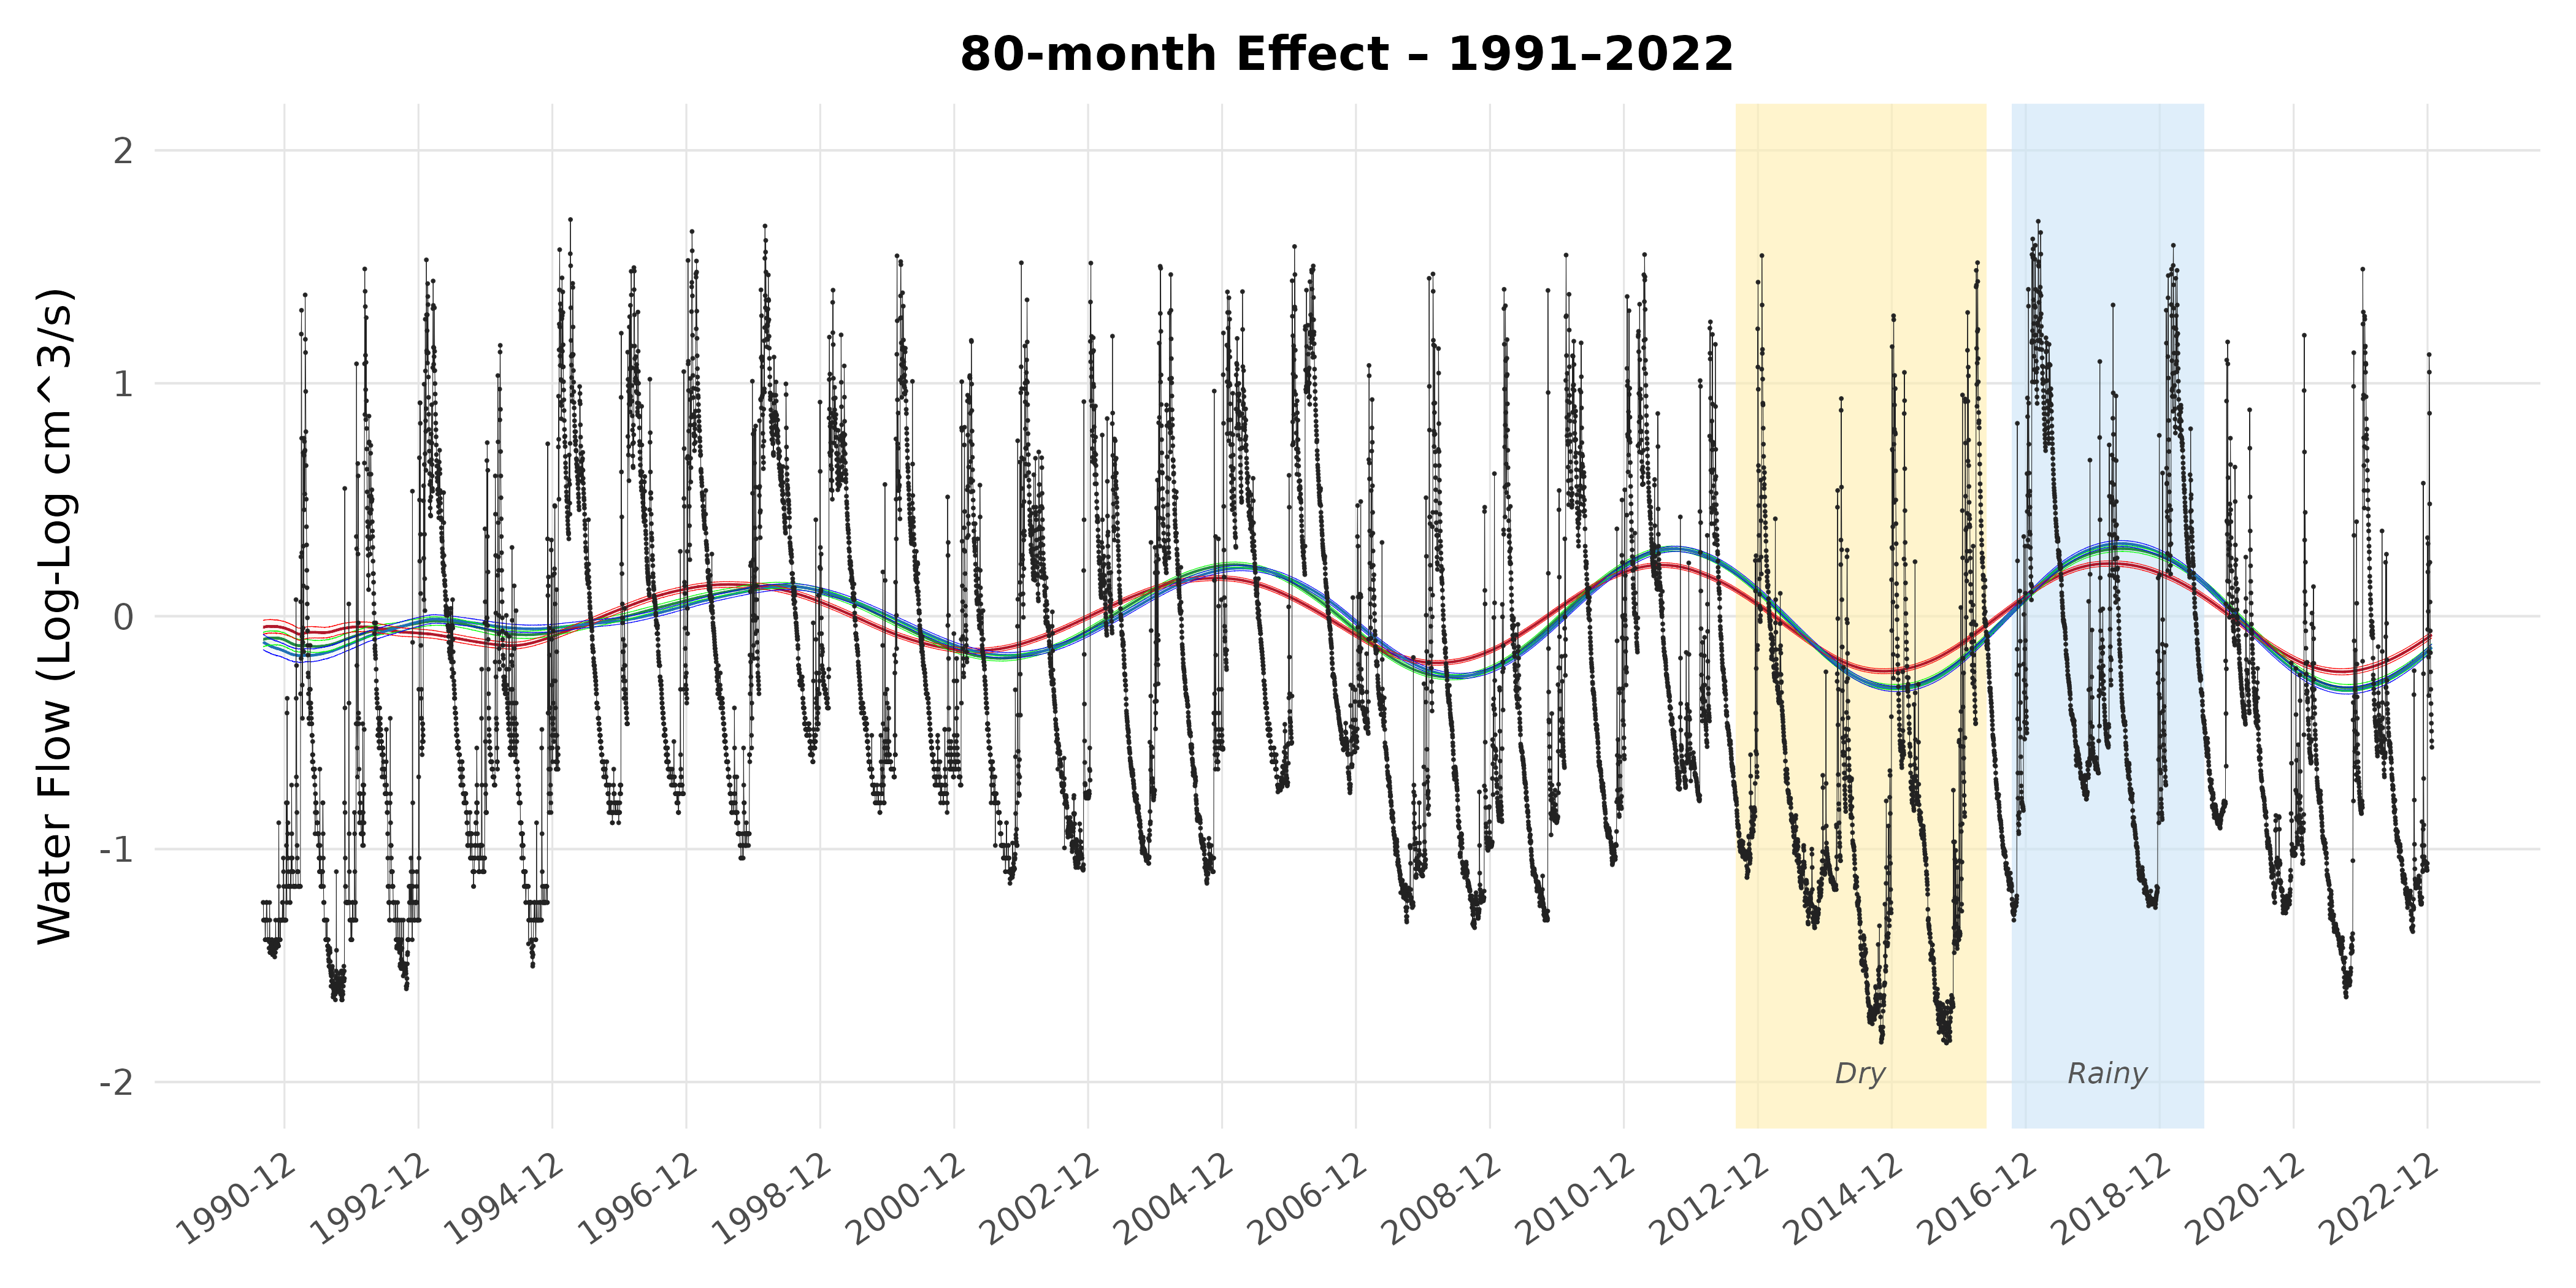
\includegraphics[width=450pt]{DISC/80_component_1991_2022.png}
\caption{
Posterior mean and 95\% credible intervals for the 80-month seasonal component of river flow from 1991 to 2022, estimated at the 5th (red), 50th (green), and 95th (blue) quantiles. Observed USGS daily flow is shown in black for reference.
}
\label{fig:80_components}
\end{figure}

Figure~\ref{fig:80_components} displays the estimated 80-month seasonality component for the 5th, 50th, and 95th quantiles from 1991 to 2022. The three quantile-specific estimates are closely aligned, indicating a stable long-term cycle across flow regimes. Notably, the component reaches its highest during the 2017–2019 wet period and its lowest through the 2012–2016 drought. This component became more regular after the early 2000s, coinciding with increased management and infrastructure interventions visible in the river flow data. These results highlight the component's value for capturing multi-year hydrological variability.

 % (see Figure~\ref{fig:sanlorenzo}, especially after the 2004 levee and floodwall reconstruction). 
 
\begin{figure}[h]
\centering
\includegraphics[width=450pt]{DISC/All_exal_2012-2016_DISC.png}
\caption{
Posterior mean and 95\% credible intervals of river flow quantiles during the dry period (2012--2016). Shown are estimates for the 5th (red), 50th (green), and 95th (blue) quantile models, along with observed daily USGS flow (black). Horizontal dashed lines mark NOAA-defined minor and major flooding thresholds.
}
\label{fig:dry_quantile}
\end{figure}

\begin{figure}[h]
\centering
\includegraphics[width=450pt]{DISC/All_exal_2017-2019_DISC.png}
\caption{
Posterior mean and 95\% credible intervals of river flow quantiles during the wet period (2017--2019). Shown are estimates for the 5th (red), 50th (green), and 95th (blue) quantile models, along with observed daily USGS flow (black). Horizontal dashed lines mark NOAA-defined minor and major flooding thresholds.
}
\label{fig:rainy_quantile}
\end{figure}

Figures~\ref{fig:dry_quantile} and \ref{fig:rainy_quantile} show posterior means and 95\% credible intervals for the 5th, 50th, and 95th quantile models during the dry (2012–2016) and wet (2017–2019) periods. In the wet period, river discharge exhibits greater variability, especially in late fall and early winter. In the winters of 2017 and 2019, the 95th quantile frequently exceeds the major flood stage threshold; in February 2017, the 5th quantile approaches the minor flood stage, consistent with observed flooding. These patterns indicate that the quantile models capture shifts in tail risk associated with high–flow episodes.

Credible bands around each individual quantile are relatively tight and stable overall, consistent with the long sample and the model’s linear dynamics. The quantile range (Q95–Q05), however, is adaptive to the different periods: it narrows during the dry period (2012–2016) and rain–free months, and widens in the wet period (2017–2019) and during late–fall/early–winter events. This widening during high–flow episodes suggests the model allocates more uncertainty when flows are volatile, aligning with precipitation–driven variability.

No quantile crossing was observed in our results, despite fitting models independently for each quantile. However, quantile crossing can still occur, particularly in smaller samples or with more volatile data. If this becomes a concern, joint model selection approaches that impose non-crossing constraints could be considered to ensure the monotonicity of quantile estimates.

\begin{table*}[htbp]
\centering
\renewcommand{\arraystretch}{1.13}
\begin{threeparttable}
\caption{Posterior Means and 95\% Credible Intervals for Covariate Effects}
\label{tab:components_23_31}
\begin{tabular*}{\textwidth}{@{\extracolsep{\fill}} l c S[table-format=-1.3] l }
\toprule
\textbf{Covariate} & \textbf{Quantile} & \textbf{Mean} & \textbf{95\% CI} \\
\midrule
\multirow{3}{*}{Precipitation}
  & 5th  & 1.945 & $[1.917,\ 1.973]$ \\
  & 50th & 2.392 & $[2.354,\ 2.429]$ \\
  & 95th & 2.946 & $[2.913,\ 2.978]$ \\
\midrule
\multirow{3}{*}{Soil Moisture}
  & 5th  & 0.115 & $[0.110,\ 0.119]$ \\
  & 50th & 0.118 & $[0.113,\ 0.124]$ \\
  & 95th & 0.253 & $[0.247,\ 0.259]$ \\
\midrule
\multirow{3}{*}{1st Principal Component}
  & 5th  & -0.084 & $[-0.087,\ -0.080]$ \\
  & 50th & -0.063 & $[-0.067,\ -0.059]$ \\
  & 95th & -0.032 & $[-0.036,\ -0.028]$ \\
\bottomrule
\end{tabular*}
\begin{tablenotes}
\item \textit{Note:} Posterior means and 95\% credible intervals $[{\rm Q2.5}, {\rm Q97.5}]$ for covariate coefficients in the transfer function, at final time $T$, for the 5th, 50th, and 95th quantile models.
\end{tablenotes}
\end{threeparttable}
\end{table*}

Table~\ref{tab:components_23_31} reports posterior means and 95\% credible intervals for the transfer–function coefficients at the 5th, 50th, and 95th quantiles (coefficients evaluated at time \(T\)). Precipitation shows the largest and increasing mean effect across quantiles \((\approx 1.95,\ 2.39,\ 2.95)\), confirming it as the primary driver of higher flows and the upper tail. 

Soil moisture is \emph{positive} at all quantiles and more pronounced in the upper tail \((\approx 0.12,\ 0.12,\ 0.25)\). A natural interpretation is antecedent wetness; wetter catchment conditions elevate baseline flow and, during storms, reduce infiltration capacity and increase runoff efficiency, thereby amplifying higher quantiles. The effect is modest at low–to–median quantiles and becomes more influential for the 95th quantile, consistent with amplification of peaks under saturated soils.

The large–scale climate factor (first principal component) remains negative and comparatively small \((\approx -0.08,\ -0.06,\ -0.03)\), with magnitude decreasing toward higher quantiles. Conditional on precipitation and soil moisture, this suggests phases of the aggregated climate indices are associated with slightly lower flows on average, but the effect is secondary relative to the physically local covariates.

Overall, the increase of both precipitation and soil–moisture effects toward the upper tail emphasize their joint role in shaping extremes. This further motivates future work on incorporating the transfer function during the forecasting period using calibrated probabilistic inputs for these covariates.


\subsection{Posterior Predictive Synthesis}
\label{subsec\:synthesis}

To obtain a single, coherent predictive distribution from several quantile-specific posterior models, we propose a synthesis strategy that utilizes localized quantile information. This approach aims to integrate the strengths of individual models, each optimized for a particular quantile, into a unified quantile function.

Let $F_t$ denote the true but unknown predictive distribution of the observation $y_t$ at time $t$. We target $L \in \mathbb{Z}_+$ distinct quantile levels $\tau_1 < \tau_2 < \dots < \tau_L$, and for each $\tau_i$, define $\hat{F}_{i,t}$ as the posterior predictive distribution from the $\text{exAL}_{\tau_i}$ model. By construction, each model is locally accurate at its respective quantile:
\[
\hat{F}_{i,t}^{-1}(\tau_i) \approx F_t^{-1}(\tau_i), \quad \forall i \in \{1, \dots, L\}.
\]

To synthesize these models, we define a unified quantile function, $(F_t^{\text{synth}})^{-1}(u)$, using piecewise linear interpolation between adjacent quantile models:
\begin{align}
(F^{\text{synth}}_t)^{-1}(u) =
\begin{cases}
\hat{F}_{1,t}^{-1}(u), & u \leq \tau_1, \\
(1 - w)\hat{F}_{i,t}^{-1}(u) + w\hat{F}_{i+1,t}^{-1}(u), & \tau_i \leq u < \tau_{i+1}, \\
\hat{F}_{L,t}^{-1}(u), & u \geq \tau_L,
\end{cases}
\label{synth_quantile}
\end{align}
where $w = \frac{u - \tau_i}{\tau_{i+1} - \tau_i}$ and $i = \max\{j : \tau_j \leq u\}$. This construction guarantees that the synthesized quantile function matches the posterior predictive quantiles at the specified levels and provides a smooth approximation between them.

The key assumption of this synthesis approach is that each quantile model provides a correctly estimated quantile at its target level, ensuring that the resulting quantile function remains monotonic. In practice, this assumption can be violated, especially since the quantile models are fit independently, which may lead to quantile crossing (e.g., $\hat{F}_{k,t}^{-1}(\tau_k) > \hat{F}_{\ell,t}^{-1}(\tau_\ell)$ for $\tau_k < \tau_\ell$) or a loss of monotonicity in the synthesized quantile function. 

To resolve quantile crossing and guarantee a globally monotonic synthesized quantile function, we implement an additional two-step correction procedure.

\paragraph{Isotonic Adjustment}  
First, we enforce monotonicity at the specified quantile levels by applying isotonic regression \citep{barlow1972}. At each time $t$, we solve the following constrained least squares problem:
\begin{align}
\mathbf{m}_t^* = \underset{m_1 \leq m_2 \leq \dots \leq m_L}{\arg\min} \sum_{i=1}^L \left( \hat{F}_{i,t}^{-1}(\tau_i) - m_i \right)^2,
\label{eq:isotonic_regression}
\end{align}
where $\hat{F}_{i,t}^{-1}(\tau_i)$ are the independently estimated posterior predictive quantiles. The solution, $\mathbf{m}_t^* = (m_{1,t}^*, \dots, m_{L,t}^*)$, provides a set of non-decreasing quantile values. We then adjust the corresponding posterior predictive distributions by shifting each posterior predictive distribution samples:
\[
y_{i,t}^{\text{adj}} = y + (m_{i,t}^* - \hat{F}_{i,t}^{-1}(\tau_i)), \quad y \sim \hat{F}_{i,t},
\]
producing adjusted distributions $F_{i,t}^{\text{adj}}$ that now satisfy $(F_{i,t}^{\text{adj}})^{-1}(\tau_i) = m_{i,t}^*$ at the target quantiles.

Using these isotonic-adjusted distributions in place of the originals, we repeat the synthesis in Eq.~\ref{synth_quantile} to produce an initial synthesized quantile function, denoted $Q_t^{\text{init}}$.

\paragraph{Monotonic Rearrangement}  
Second, to enforce monotonicity across the entire quantile domain (not just at the grid points), we apply monotonic rearrangement as described by \citet{chernozhukov2010}. This is accomplished by:
\begin{enumerate}
    \item Evaluating $Q_t^{\text{init}}$ on a dense grid $\{u_k = k/(M+1)\}_{k=1}^M$.
    \item Sorting the resulting values to obtain $\mathbf{q}_t^{\uparrow} = \operatorname{sort}(Q_t^{\text{init}}(u_1), \dots, Q_t^{\text{init}}(u_M))$.
    \item Defining the final synthesized quantile function $Q_t$ via linear interpolation of the pairs $\{(u_k, q_{t,k}^{\uparrow})\}_{k=1}^M$.
\end{enumerate}
This rearrangement step ensures strict monotonicity of the final synthesized quantile function $Q_t$, with finite-sample theoretical guarantees for quantile estimation.

In our specific application, the corrected posterior predictive synthesis yielded results nearly identical to the uncorrected synthesis described earlier, primarily due to the absence of quantile crossing. Consequently, the explicit monotonicity corrections had limited practical impact.

\begin{figure}[h]
\centering
\includegraphics[width=450pt]{DISC/posterior_samples_valid.png}
\caption{
Synthesized posterior predictive distribution for river flow (log-log scale, cm$^3$/s) at the San Lorenzo River. Observed USGS measurements before December 25, 2022, are shown in green; unobserved future measurements are shown in red. Retrospective analyses (gray) are shown before December 25, and ensemble forecasts (gray) from ECMWF and NWS are shown after this date. Horizontal dashed lines indicate NOAA-defined minor and major flooding thresholds. The thin black lines shown along with the synthesized distribution (pink) correspond to the quantiles of the synthesized distribution (percentiles: 0.05, 0.20, 0.35, 0.5, 0.65, 0.8, 0.95). 
}
\label{fig:synth1}
\end{figure}
Figure~\ref{fig:synth1} shows the synthesized posterior predictive distribution obtained by integrating observed USGS measurements, retrospective analyses, and ensemble forecasts, both before and after December 25, 2022. Retrospective analyses (from ECMWF and NWS) and ensemble forecasts are displayed as gray curves, illustrating the spread and uncertainty from external forecast products. Observed USGS measurements available prior to December 25 are shown in green, whereas unobserved future measurements (after December 25) are presented in red. Horizontal dashed lines indicate NOAA-defined minor and major flooding thresholds. The forecast horizon covers 28 days after the cutoff date, allowing direct comparison with subsequently observed river flows. The results indicate that, as of December 25, a marked shift in hydrological conditions was forecasted, with the upper quantiles remaining consistently above the major flood threshold. Such a signal would likely prompt the issuance of a flood warning for the following week. Not surprisingly, precipitation emerges as a dominant driver of these projected flows; however, some overestimation is apparent, reflecting the inherent difficulty of producing accurate precipitation forecasts, particularly for amounts at lead times relevant to flood risk management.

\begin{figure}[h]
\centering
\includegraphics[width=450pt]{DISC/posterior_samples_counter_valid.png}
\caption{
Idealized benchmark synthesized posterior predictive distribution for river flow (log-log scale, cm$^3$/s), based only on historical observed USGS measurements. Observed measurements before December 25, 2022, are shown in green, and unobserved future measurements are shown in red. No retrospective analyses or ensemble forecasts are included. Horizontal dashed lines indicate NOAA-defined minor and major flooding thresholds. The thin black lines shown along with the synthesized distribution (pink) correspond to the quantiles of the synthesized distribution (percentiles: 0.05, 0.20, 0.35, 0.5, 0.65, 0.8, 0.95). 
}
\label{fig:synth2}
\end{figure}

Figure~\ref{fig:synth2} presents an alternative, idealized benchmark synthesized distribution obtained by using only historical USGS measurements, excluding retrospective analyses and ensemble forecasts. This scenario assumes perfect future knowledge of covariate values and no forecast uncertainty—conditions unattainable in operational settings. Comparing this idealized benchmark with the main synthesized distribution in Figure~\ref{fig:synth1} highlights the practical value of incorporating ensemble forecasts and external data sources, even when those inputs are affected by the limitations and uncertainties associated with precipitation prediction. The thin black lines shown along with the synthesized distribution (pink) correspond to the quantiles of the synthesized distribution (percentiles: 0.05, 0.20, 0.35, 0.5, 0.65, 0.8, 0.95). 

\section{Conclusions}
\label{sec5}

This study presents a Bayesian  quantile-based framework for historical analysis and synthesis of river flow forecasts, integrating information from direct observations, retrospective analyses, and ensemble forecast products. The approach is designed as a practical, interpretable forecasting tool with the ability to quantify and propagate uncertainty at multiple quantile levels, using physically meaningful model components for a forecasting period. 

Methodologically, the primary contributions are twofold: (i) an adaptation of variational Bayes inference for the extended dynamic quantile linear model, using Laplace delta approximations to enable scalable learning of non-conjugate parameters; and (ii) the explicit modeling of discrepancies between observed river flow and retrospective analyses, enabling dynamic correction of ensemble forecasts. The framework also introduces a post-processing synthesis strategy to combine independently fitted quantile models into a coherent posterior predictive distribution, with monotonicity adjustments to ensure consistency.

Empirically, application to the San Lorenzo River system demonstrates that the model can identify and adapt to both extreme and routine flow regimes, including significant infrastructure interventions and hydrological shifts. The dynamic bands generated between quantile estimates are responsive to periods of heightened variability, and no quantile crossing was observed. The physically interpretable model structure, incorporating trend, seasonality, and covariate effects, provides practical insight into the river’s dynamics.

It is important to note that the model’s success is conditional on the quality and compatibility of the input products, as well as on structural assumptions regarding discrepancy dynamics and covariate effects. The exclusion of the transfer function during the forecast period is a particular limitation in this context, given its central role in the system's dynamic.

Looking forward, some directions include joint model selection to discourage quantile crossing, the development of nonlinear or more expressive dynamics, and the inclusion of spatial correlations. The proposed framework remains broadly applicable to other settings in which ensemble and retrospective forecast products are available, particularly where interpretability and uncertainty quantification are central concerns.

In summary, this work advances the probabilistic modeling of river flow by providing a scalable, interpretable framework for synthesizing historical and forecast information at multiple quantile levels.




\section*{Acknowledgments}

This work is part of the Ph.D. dissertation of Antonio Aguirre, as part of 
the program on statistical science at the University of
California Santa Cruz. The work was supported in part by the National Science
Foundation grant MMS2050012.

%\subsection*{Author contributions}

%\subsection*{Financial disclosure}

%None reported.

%\subsection*{Conflict of interest}

%The authors declare no potential conflict of interests.

\clearpage


\appendix

\section{Markov Chain Monte Carlo Algorithms}
\begin{algorithm}
\caption{MCMC Algorithm}\label{alg1}
\begin{algorithmic}

\State \textbf{Notation:}
\State  \(
A^j = A(\gamma^j;p_0), \quad B^j = B(\gamma^j;p_0), \quad C^j = C(\gamma^j;p_0), \text{ as defined in Section~\ref{subsec:exal}}
\)
\vspace{0.1cm}
\hline
\vspace{0.1cm}


\State \textbf{Step 0: Set initial values} and sample size $N$.
\State Initialize $\{ (v^j)^{(0)}_{1:T}$, $(s^j)^{(0)}_{1:T}$, $(\boldsymbol{\alpha})^{(0)}_{1:T}, $(\sigma^j)^{(0)}$, $(\gamma^j)^{(0)}\}_{j=0}^J$
\For{$n = 1$ to $N$}
    \State \textbf{Step 1: Update $\boldsymbol{\alpha}_t$}
    \State Use Algorithm~\ref{alg:Alg2}
    \For{$j = 0$ to $J$}
        \State \textbf{Step 2: Update $v^j_t$}
        \For{$t = 1$ to $T$}
            \State Sample $(v^j_t)^{(n)} \sim \mathcal{GIG}(a^j_t, b^j_t, c^j_t)$
            \State $a^j_t = \frac{1}{2}$
            \State $b^j_t = \frac{1}{(\sigma^j)^{(n-1)}}\left[ \frac{((A^j)^2)^{(n-1)}}{(B^j)^{(n-1)}}+2\right]$
            \State $c^j_t = \frac{1}{(\sigma^j)^{(n-1)} (B^j)^{(n-1)}}\left[y_t^j -\textbf{h}_{t,j+1}' \boldsymbol{\alpha}^{(n)}_t -(C^j)^{(n-1)} (\sigma^j)^{(n-1)} |(\gamma^j)^{(n-1)}| (s^j_t)^{(n-1)} \right]^2$
        \EndFor
        \For{$t = T+1$ to $T+K_{(1)}$}
            \State Sample $(v^j_t)^{(n)} \sim \mathcal{GIG}(a^j_t, b^j_t, c^j_t)$
            \State $a^j_t = \frac{1}{2}$
            \State $b^j_t = \frac{1}{(\sigma^j)^{(n-1)}}\left[ \frac{((A^j)^2)^{(n-1)}}{(B^j)^{(n-1)}}+2\right]$
            \State $c^j_t = \frac{1}{(\sigma^j)^{(n-1)} (B^j)^{(n-1)}}\left[y_t^j -\textbf{h}_{t,j+1}' \boldsymbol{\alpha}^{(n)}_t -(C^j)^{(n-1)} (\sigma^j)^{(n-1)} |(\gamma^j)^{(n-1)}| (s^j_t)^{(n-1)} \right]^2$
        \EndFor

        \State \textbf{Step 3: Update $s^j_t$}
        \For{$t = 1$ to $T$}
            \State Sample $(s^j)^{(n)}_t \sim \mathcal{N}^+(m^j_t, \lambda^j_t)$
            \State $\lambda^j_t =  \left[\frac{\big((C^j)^{(n-1)}\gamma^{(n-1)} \big)^2(\sigma^j)^{(n-1)}}{(B^j)^{(n-1)}(v^j_t)^{(n)}}+1\right]$
            \State $m^j_t =  \lambda^j_t \left[\frac{(C^j)^{(n-1)}|\gamma^{n-1}|(y_t^j -\textbf{h}_{t,j+1}' \boldsymbol{\alpha}^{(n)}_t - (A^j)^{(n-1)} (v^j_t)^{(n)})}{(B^j)^{(n-1)}(v^j_t)^{(n)}}\right]$
        \EndFor

        \State \textbf{Step 4: Update $\sigma^j$}
        \State Sample $(\sigma^j)^{(n)} \sim \mathcal{GIG}(a^j_t, b^j_t, c^j_t)$
        \State $a^j_t = -(1.5T + a_{\sigma^j})$
        \State $b^j_t = \sum_{t=1}^T \frac{1}{(B^j)^{(n-1)} (v^j_t)^{(n)}} \left((C^j)^{(n-1)} |(\gamma^j)^{(n-1)}| (s^j_t)^{(n)} \right)^2$
        \State $c^j_t = \sum_{t=1}^T \frac{1}{(B^j)^{(n-1)} (v^j_t)^{(n)}}\big(y_t^j -\textbf{h}_{t,j+1}' \boldsymbol{\alpha}^{(n)}_t - (A^j)^{(n-1)} (v^j_t)^{(n)}\big)^2 + 2 \sum_{t=1}^T  (v^j_t)^{(n)} + 2 b_{\sigma^j}$

        \State \textbf{Step 5: Update $\gamma^j$}
        \State Implement Metropolis-Hastings (MH)
    \EndFor
\EndFor

\end{algorithmic}
\end{algorithm}

\begin{algorithm}
\caption{MCMC - Forward Filtering Backward Sampling (FFBS)}
\label{alg:Alg2}
\begin{algorithmic}

\State \textbf{Notation:}
\State  $\mathbf{H}_t$, $\mathbf{D}_t$ and $\boldsymbol{\Lambda}_t$ are as defined in Section~\ref{subsec:retrospective}
\State $\mathbf{M}_t= \mathbf{C} \odot  \mathbf{\sigma} \odot | \mathbf{\gamma} | \odot \mathbf{s}_t + \mathbf{A} \odot \mathbf{v}_t$, \quad $\mathbf{O}_t= \sqrt{\mathbf{B} \odot \mathbf{v}_t} \odot Diag
(\mathbf{\sigma}) \sqrt{\mathbf{B} \odot \mathbf{v}_t} \odot \mathbf{\sigma}$
\State  \(
\mathbf{A} = \big[ A(\gamma^j;p_0)   \big], \quad \mathbf{B} = \big[  B(\gamma^j;p_0)  \big], \quad \mathbf{C} = \big[ C(\gamma^j;p_0)   \big] \), \text{ as defined in Section~\ref{subsec:exal}}
\State \( \mathbf{v}_t = \big[  v^j_t   \big], \quad  \mathbf{s}_t = \big[ 
s^j_t  \big] , \quad \mathbf{\sigma} = \big[ \sigma^j  \big]
\)
\State \text{where } \odot \text{ is the Hadamard product}
\vspace{0.1cm}
\hline
\vspace{0.1cm}

\State \textbf{Step 1: Forward Filtering}
\For{$t = 1$ to $T$}
    \State Compute Prior moments:
    \State $\mathbf{a}_t = \mathbf{D}_t \mathbf{m}_{t-1}$
    \State $\mathbf{R}_t = \mathbf{D}_t \mathbf{C}_{t-1} \mathbf{D}_t' +  \boldsymbol{\Lambda}_t$

    \State One-step-ahead forecast:
    \State $\mathbf{f}_t = \mathbf{H}_t' \mathbf{a}_t + \mathbf{M}_t$
    \State $\mathbf{Q}_t = \mathbf{H}_t' \mathbf{R}_t \mathbf{H}_t + \mathbf{O}_t$
    
    \State Compute Posterior moments:
    \State $\mathbf{m}_t = \mathbf{a}_t + \mathbf{R}_t \mathbf{H}_t \mathbf{Q}_t^{-1}(\mathbf{Y}_t - \mathbf{f}_t)$
    \State $\mathbf{C}_t = \mathbf{R}_t - \mathbf{R}_t \mathbf{H}_t \mathbf{Q}_t^{-1} \mathbf{H}_t' \mathbf{R}_t$
\EndFor

\State \textbf{Step 2: Backward Sampling}
\For{$t = T$ down to $0$}
    \If{$t = T$}
        \State Sample $\boldsymbol{\theta}_T | D_T \sim \mathcal{N}(\mathbf{m}_T, \mathbf{C}_T)$
    \Else
        \State Compute Retrospective moments:
        \State $\mathbf{m}_t^s = \mathbf{m}_t + \mathbf{C}_t \mathbf{G}_{t+1}' \mathbf{R}_{t+1}^{-1} (\boldsymbol{\theta}_{t+1} - \mathbf{a}_{t+1})$
        \State $\mathbf{C}_t^s = \mathbf{C}_t - \mathbf{C}_t \mathbf{G}_{t+1}' \mathbf{R}_{t+1}^{-1} \mathbf{D}_{t+1} \mathbf{C}_t$
        
        \State Sample $\boldsymbol{\theta}_t | D_T \sim \mathcal{N}(\mathbf{m}_t^s, \mathbf{C}_t^s)$
    \EndIf
\EndFor

\end{algorithmic}
\end{algorithm}

 \clearpage


\section{Variational Bayes Algorithms}

\begin{algorithm}
\caption{Variational Bayes (VB) Algorithm}
\label{alg:Alg3}
\begin{algorithmic}

\State \textbf{Notation:}
\State  $\left\langle g(\xi) \right\rangle = \mathbb{E}_\xi\left[ g(\xi) \right]$
\State  \(
A^j = A(\gamma^j;p_0), \quad B^j = B(\gamma^j;p_0), \quad C^j = C(\gamma^j;p_0), \text{ as defined in Section~\ref{subsec:exal}}
\)
\vspace{0.1cm}
\hline
\vspace{0.1cm}

\State \textbf{Step 0: Set initial values}

\While{$\text{ELBO}_k > \text{tol}$}
    \State \textbf{Step 1: Update $r(\boldsymbol{\alpha}_t)=\mathcal{N}(m^{(k)}_t,C^{(k)}_t)$}
    \State Use Algorithm~\ref{alg:Alg4}

    \For{$j = 0$ to $J$}
        \State \textbf{Step 2: Update $r(v^j_t)=\mathcal{GIG}(a_t^{j,(k)},b_t^{j,(k)},c_t^{j,(k)})$}
        \For{$t = 1$ to $T$}
            \State $a_t^{j,(k)} = \frac{1}{2}$
            \State $b_t^{j,(k)} = \left\langle \frac{A^2}{\sigma^j B^j} \right\rangle^{(k-1)} + 2 \left\langle \frac{1}{\sigma^j} \right\rangle^{(k-1)}$
            \State $c_t^{j,(k)} = \left\langle \frac{1}{\sigma^j B^j} \right\rangle^{(k-1)} \Big[ (y_t^j)^2 - 2y_t^j \left\langle  \mathbf{h}_{t,j+1} \boldsymbol{\alpha}_t \right\rangle^{(k)} + \left\langle (  \mathbf{h}_{t,j+1} \boldsymbol{\alpha}_t )^2 \right\rangle^{(k)} \Big]$
            \State $\quad \quad -2 \left\langle s^j_t \right\rangle^{(k-1)} \left\langle \frac{C^j|\gamma^j|}{B^j} \right\rangle^{(k-1)} \Big[ y_t^j - \left\langle  \mathbf{h}_{t,j+1} \boldsymbol{\alpha}_t \right\rangle^{(k)} \Big]$
            \State $\quad \quad + \left\langle (s^j_t)^2 \right\rangle^{(k-1)} \left\langle \frac{(C^j)^2\sigma^j|\gamma^j|^2}{B^j} \right\rangle^{(k-1)}$
        \EndFor

        \State \textbf{Step 3: Update $r(s^j_t)=\mathcal{N}^+(\eta^{j,(k)},\lambda^{j,(k)})$}
        \For{$t = 1$ to $T$}
            \State $\lambda^{j,(k)} = \Big[ 1+\left\langle \frac{(C^j)^2 \sigma^j |(\gamma^j)|^2}{B^j} \right\rangle^{(k-1)} \left\langle \frac{1}{v^j_t} \right\rangle^{(k)} \Big]^{-1}$
            \State $\eta^{j,(k)} = \lambda^{j,(k)}  \Big[ \left\langle \frac{C^j |\gamma^j|}{B^j} \right\rangle^{(k-1)} \left\langle \frac{1}{v^j_t} \right\rangle^{(k)} \Big( y_t^j - \left\langle  \mathbf{h}_{t,j+1} \boldsymbol{\alpha}_t \right\rangle^{(k)} \Big) - \left\langle \frac{C^j |\gamma^j| A^j}{B^j} \right\rangle^{(k-1)} \Big]$
        \EndFor

        \State \textbf{Step 4: Update $r(\gamma^j, \sigma^j )$}
        \State Approximate via VB-LD, as described in Section~\ref{subsec:postinf}
    \EndFor
\EndWhile

\end{algorithmic}
\end{algorithm}

\begin{algorithm}
\caption{VB-Filtering and VB-Smoothing}
\label{alg:Alg4}
\begin{algorithmic}

\State \textbf{Notation:}
\State $\left\langle g(\xi) \right\rangle = \mathbb{E}_\xi\left[ g(\xi) \right]$
\State  $\mathbf{H}_t$, $\mathbf{D}_t$ and $\boldsymbol{\Lambda}_t$ are as defined in Section~\ref{subsec:retrospective}
\State $\mathbf{M}_t= \mathbf{C} \odot  \mathbf{\sigma} \odot | \mathbf{\gamma} | \odot \mathbf{s}_t + \mathbf{A} \odot \mathbf{v}_t$, \quad $\mathbf{O}_t= \sqrt{\mathbf{B} \odot \mathbf{v}_t} \odot Diag
(\mathbf{\sigma}) \sqrt{\mathbf{B} \odot \mathbf{v}_t} \odot \mathbf{\sigma}$
\State  \(
\mathbf{A} = \big[ \left\langle A(\gamma^j;p_0)  \right\rangle \big], \quad \mathbf{B} = \big[ \left\langle B(\gamma^j;p_0)  \right\rangle \big], \quad \mathbf{C} = \big[ \left\langle C(\gamma^j;p_0)  \right\rangle \big] \), \text{ as defined in Section~\ref{subsec:exal}}
\State \( \mathbf{v}_t = \big[ \left\langle v^j_t  \right\rangle \big], \quad  \mathbf{s}_t = \big[ \left\langle
s^j_t  \right\rangle \big] , \quad \mathbf{\sigma} = \big[ \left\langle \sigma^j  \right\rangle \big]
\)
\State \text{where } \odot \text{ is the Hadamard product}
\vspace{0.1cm}
\hline
\vspace{0.1cm}

\State \textbf{Step 1: Forward Filtering}
\For{$t = 1$ to $T$}
    \State Compute Prior moments:
    \State $\mathbf{a}_t = \mathbf{D}_t \mathbf{m}_{t-1}$
    \State $\mathbf{R}_t = \mathbf{D}_t \mathbf{C}_{t-1} \mathbf{D}_t' +  \boldsymbol{\Lambda}_t$

    \State One-step-ahead forecast:
    \State $\mathbf{f}_t = \mathbf{H}_t'\mathbf{a}_t + \mathbf{M}_t$
    \State $\mathbf{Q}_t = \mathbf{H}_t'\mathbf{R}_t\mathbf{H}_t + \mathbf{O}_t$
    
    \State Compute Posterior moments:
    \State $\mathbf{m}_t = \mathbf{a}_t + \mathbf{R}_t \mathbf{H}_t \mathbf{Q}_t^{-1}(\mathbf{Y}_t - \mathbf{f}_t)$
    \State $\mathbf{C}_t = \mathbf{R}_t - \mathbf{R}_t \mathbf{H}_t \mathbf{Q}_t^{-1} \mathbf{H}_t' \mathbf{R}_t$
\EndFor

\State \textbf{Step 2: Backward Smoothing}
\For{$t = T$ down to $1$}
    \If{$t = T$}
        \State Set $r^{(k+1)}(\boldsymbol{\theta}_T) := \mathcal{N}(\mathbf{m}_T^s, \mathbf{C}_T^s)$
        \State $\mathbf{m}_T^s = \mathbf{m}_T$
        \State $\mathbf{C}_T^s = \mathbf{C}_T$
    \Else
        \State Compute Smoothing moments:
        \State $r^{(k+1)}(\boldsymbol{\theta}_t) := \mathcal{N}(\mathbf{m}_t^s, \mathbf{C}_t^s)$
        \State $B_t = \mathbf{C}_t \mathbf{D}_{t+1}' \mathbf{R}_{t+1}^{-1}$
        \State $\mathbf{m}_t^s = \mathbf{m}_t + \mathbf{B}_t (\mathbf{m}_{t+1}^s - \mathbf{a}_{t+1})$
        \State $\mathbf{C}_t^s = \mathbf{C}_t + \mathbf{B}_t (\mathbf{C}_{t+1}^s - \mathbf{R}_{t+1}) \mathbf{B}_t'$
    \EndIf
\EndFor


\end{algorithmic}
\end{algorithm}


\nocite{*}% 

\clearpage

\bibliography{wileyNJD-APA}%

\section*{Author Biography}

\begin{biography}{
\includegraphics[width=60pt,height=70pt  ]{empty}}{\textbf{Author Name.} This is sample author biography text this is.}
\end{biography}

\end{document}
